\documentclass[sensors,article,submit,moreauthors,pdftex]{Definitions/mdpi}

\firstpage{1}
\makeatletter
\setcounter{page}{\@firstpage}
\makeatother
\pubvolume{xx}
\issuenum{1}
\articlenumber{0}
\pubyear{2026}
\copyrightyear{2026}
\setlength{\headheight}{24.19pt}
\usepackage{amsmath,amssymb,amsfonts}
\usepackage{algorithmic}
\usepackage{graphicx}
\usepackage{textcomp}
\usepackage{xcolor}
\usepackage{booktabs}
\usepackage{colortbl}
\definecolor{hdrblue}{RGB}{30,80,140}
\definecolor{rowA}{RGB}{240,245,255}
\definecolor{prevbest}{RGB}{255,248,210}
\definecolor{oursgood}{RGB}{220,245,220}
\definecolor{oursbest}{RGB}{180,230,180}
\usepackage{array}
% --- revision markup: all text added or changed in this revision ---
\newcommand{\rev}[1]{\textcolor{blue}{#1}}
\usepackage{multirow}
\usepackage{subcaption}
\usepackage{float}
\usepackage{placeins}

\usepackage{tikz}
\usetikzlibrary{positioning,arrows.meta,shapes.geometric,fit,calc,shadows,backgrounds}

\usepackage{lastpage}

\usepackage{pgfplots}
\pgfplotsset{compat=1.18}
\usepgfplotslibrary{groupplots}

\graphicspath{{figs/}}

% --- MDPI Frontmatter ---
\Title{SpaSE-UNet3D: Sensor-Driven Wildfire Detection and Progression Prediction from VIIRS Multispectral Imagery}

\Author{Nikolaos Mavros $^{1}$ and Dimitrios Katsaros $^{1,*}$}

\AuthorNames{Nikolaos Mavros and Dimitrios Katsaros}

\address{$^{1}$ \quad Department of Electrical and Computer Engineering,
University of Thessaly, Volos, Greece;
nmavros@uth.gr (N.M.); dkatsar@uth.gr (D.K.)}

\corres{Correspondence: dkatsar@uth.gr}

\abstract{Timely wildfire monitoring depends critically on optical and
thermal infrared sensor observations from spaceborne instruments. The
Visible Infrared Imaging Radiometer Suite (VIIRS) aboard Suomi-NPP and
NOAA-20 is the primary sensor system underlying the TS-SatFire benchmark
(2025), which consolidates multispectral VIIRS image stacks for three
tasks: Active Fire (AF) detection, Burned Area (BA) mapping, and Fire
Progression (FP) prediction. We make two contributions. First, a
\rev{systematic label-quality audit across all tasks and splits reveals that
many fires lack ground-truth annotations: 18 training fires
and 2 test fires are excluded for AF, and the two unannotated test fires cannot
be scored by any model. We further show that the reference evaluation of this
benchmark differs from an independently implemented one in eight respects, and
that these differences move F1 by up to 0.10 on fixed model weights---several
times the spread separating the published baselines from one another. Published
figures are therefore not directly comparable to independently computed values.}
We also document the BA label encoding in the released GeoTIFFs---a 
prerequisite for downstream modelling; \rev{the BA task is used for auditing
only and no BA model is trained.} Second, we propose
SpaSE-UNet3D, a spatial Squeeze-and-Excitation 3D UNet. By using
spatial-only $(1,3,3)$ convolutions, our architecture avoids temporal mixing 
\rev{in the convolutional path}
on short observation windows, while utilizing SE channel attention to reweight
the VIIRS spectral bands dynamically. \rev{Under the protocol defined in this
paper, SpaSE-UNet3D reaches F1\,=\,$0.8549 \pm 0.0005$ on AF at TS\,=\,2 and
F1\,=\,$0.3843 \pm 0.0392$ on FP over the full 24-fire test set, using two-day
observation windows against the published baselines' six, at 32.9\,M and
24.3\,M parameters and under 12 hours of total training on a single GPU.} Code and
results are publicly available.}

\keyword{wildfire detection; VIIRS; active fire; fire progression; 3D U-Net; squeeze-and-excitation; remote sensing; deep learning; satellite imagery; label quality audit}

\begin{document}

\label{LastPage}

\maketitle


%%=============================================================
\section{Introduction}
%%=============================================================

Wildfires are increasingly destructive across temperate and boreal
biomes, and timely automated detection of active fire fronts, burned
extents, and near-term fire progression is essential for operational
response. Satellite-borne optical and thermal infrared sensors are
the primary mechanisms enabling this monitoring at continental
scale, with daily or twice-daily revisit and spectral bands
specifically calibrated for fire radiometry. Among spaceborne 
systems, the Visible Infrared Imaging Radiometer Suite (VIIRS)
aboard Suomi-NPP and NOAA-20 stands out: it provides 22 
bands spanning the visible, near-infrared, and thermal infrared
spectrum, of which five imaging-resolution bands at 375\,m are
directly exploited for active fire detection~\cite{schroeder2014new}.
Barmpoutis et~al.~\cite{barmpoutis2020review} survey the full
landscape of optical sensor systems for early fire detection,
distinguishing terrestrial, airborne, and spaceborne 
architectures and confirming that VIIRS and MODIS spaceborne
sensors provide the most operationally scalable coverage for
large-scale wildfire monitoring. \rev{Alongside these learned approaches,
index-based methods applied to moderate-resolution optical sensors remain
widely used for post-fire burned-area assessment: spectral indices such as the
Normalized Burn Ratio have been applied to Landsat~8 imagery to delineate
burning areas in protected forest~\cite{laosuwan2023inspection}, and
comparable index-based procedures using Sentinel-2 data have been used to
quantify burned extents in wildlife sanctuaries over multi-year
periods~\cite{uttaruk2022burned}. These methods provide the operational
baseline against which learned approaches are measured.}

The recently released TS-SatFire dataset~\cite{zhao2025tssatfire}
consolidates several years of VIIRS  observations into a
common benchmark for three wildfire tasks: Active Fire (AF) pixel
detection, Burned Area (BA) mapping, and Fire Progression (FP)
prediction. Each fire event is represented as a temporal stack of
multispectral VIIRS sensor images, with up to eight daytime
reflectance and thermal  channels plus complementary
nighttime thermal  bands — a design motivated by the
demonstrated value of combining daytime optical sensor observations
with nighttime thermal infrared  data for round-the-clock
fire tracking~\cite{chiang2019mapping}. The dataset paper reports
results for 11 baselines ranging from 2D U-Nets~\cite{ronneberger2015unet}
to 3D transformer variants~\cite{hatamizadeh2022swin,hatamizadeh2022unetr},
using sensor temporal stacks of up to TS\,=\,6 days. The strongest
published AF baseline is SwinUNETR-3D at TS\,=\,2 with F1\,=\,0.823;
the strongest published FP baseline is U-Net-3D at TS\,=\,6 with
F1\,=\,0.374.

\rev{The benchmark has been used to rank eleven architectures against one
another, but neither the completeness of its labels nor the evaluation
procedure used to produce those rankings has been examined. Both, we find,
materially affect the reported ordering. Our contribution is therefore twofold,
and we state the ordering explicitly: the primary contribution is documentation
of the benchmark's evaluation protocol and label quality; the secondary
contribution is an architecture, presented on efficiency grounds.}

In this work we revisit TS-SatFire with two goals. The first is to
examine the sensor data itself. We observe during initial experiments
that recall is systematically capped at approximately 0.80 for models
that otherwise perform well, which is inconsistent with the near-equal
precision values. A systematic audit of every fire in every split
reveals a substantial number of fires with entirely missing 
labels, across all three tasks; training on unaudited data
therefore incurs a penalty that is fully attributable to the data and
not to the model. The audit findings are themselves a standalone
contribution and are required for any future work on this benchmark.

The second goal is architectural. The TS-SatFire sensor input is
very short: operational constraints and paper conventions favour
temporal windows of 1--2 days for AF and 2--6 days for FP. On such
short windows, the implicit temporal prior that motivates full 3D
convolutions in video understanding~\cite{tran2018closer,qiu2017learning}
or volumetric medical imaging~\cite{cciccek20163d} is \rev{not obviously
justified}: there is \rev{little} inter-day sensor signal to decorrelate.
Prior work in action recognition has shown that factorising 3D
convolutions into separate spatial and temporal components yields
better accuracy with fewer parameters~\cite{tran2018closer,qiu2017learning},
and \rev{our design tests this intuition at its limit} by removing temporal
mixing inside the residual blocks entirely. We propose SpaSE-UNet3D,
a spatial Squeeze-and-Excitation 3D UNet that explicitly uses
$(1,3,3)$ convolutions in every residual block, so that the temporal
dimension is preserved but never mixed across days. The block
further uses SE~\cite{hu2018squeeze} channel attention to reweight
the VIIRS multispectral sensor bands per spatial context.
Task-specific variants add an ASPP~\cite{chen2017rethinking,chen2018encoder}
bottleneck and a 27-channel auxiliary-feature input for
fire progression.

\rev{We evaluate SpaSE-UNet3D on both the AF and FP tasks under the
evaluation protocol defined in Section~\ref{sec:experiments}. On AF it reaches
F1\,=\,$0.8549 \pm 0.0005$ at TS\,=\,2 on the 15 annotated test fires, and
on FP F1\,=\,$0.3843 \pm 0.0392$ at TS\,=\,2 over the full 24-fire test set,
in both cases using two-day observation windows where the published baselines
use six, and training in under 12 hours on a single NVIDIA~T4 accelerator. We
do not present these figures as improvements over the published baselines:
as Section~\ref{sec:experiments} establishes, the two sets of numbers are not
computed under a common protocol.} We treat the BA task as audit-only: the
audit itself is a dataset contribution, but we do not present a learned BA
model.

\rev{The objectives of this study are: (i)~to quantify the completeness of
the TS-SatFire labels across all three tasks and splits, and to document the
burned-area encoding required to use them; (ii)~to determine whether published
baseline figures and independently computed figures measure the same quantity,
and to isolate the contribution of each difference; (iii)~to develop an
architecture suited to the short observation windows the benchmark provides,
and to characterise its computational cost as well as its accuracy; and
(iv)~to establish the run-to-run variability of both tasks, so that reported
differences can be interpreted against measurement noise.}

The rest of the paper is organised as follows.
Section~\ref{sec:related} reviews related work.
Section~\ref{sec:dataset} describes the TS-SatFire dataset.
Section~\ref{sec:audit} presents our label-quality audit.
Section~\ref{sec:method} details the SpaSE-UNet3D architecture
and its task-specific variants.
Section~\ref{sec:experiments} reports the experimental protocol
and results.
Section~\ref{sec:discussion} discusses the findings and
Section~\ref{sec:conclusion} concludes.

%%=============================================================
\section{Related Work}
\label{sec:related}
%%=============================================================

\paragraph*{Wildfire remote sensing with deep learning.} Early work on active fire detection from satellite imagery used per-pixel thresholds on thermal bands, typically VIIRS band I4 or the MODIS analogue~\cite{giglio2016collection,schroeder2014new}. Deep learning approaches in the last five years have moved to segmentation networks operating on multi-band VIIRS or Sentinel-2 stacks~\cite{pinto2020deep}, and more recently to 3D and transformer architectures that incorporate temporal context~\cite{moskolai2021application}. Huot et~al.~\cite{huot2022next} released the Next Day Wildfire Spread benchmark, with a related but coarser problem formulation than TS-SatFire. Zhao and Ban~\cite{zhao2025tssatfire} provide the most comprehensive comparison to date, benchmarking 12 architectures spanning U-Net~\cite{ronneberger2015unet}, Attention U-Net~\cite{oktay2018attention}, UNETR~\cite{hatamizadeh2022unetr}, SwinUNETR~\cite{hatamizadeh2022swin}, and recurrent encoders on a unified TS-SatFire benchmark. Their results motivate our comparisons throughout.

\paragraph*{Factorised spatiotemporal convolutions.} Tran et~al.~\cite{tran2018closer} and Qiu et~al.~\cite{qiu2017learning} showed that factorising 3D convolutions into separate spatial $(1, k, k)$ and temporal $(k, 1, 1)$ stages outperforms full $(k, k, k)$ kernels in video classification, with fewer parameters. SpaSE-UNet3D extends this principle to its extreme on short ($T \leq 2$) windows by retaining only the spatial component, supported by our ablations.

\paragraph*{Attention in U-Nets.} Squeeze-and-Excitation~\cite{hu2018squeeze} adds a lightweight channel-wise attention module that globally pools feature maps and produces per-channel gating weights. Roy et~al.~\cite{roy2018concurrent} extended this with concurrent spatial-channel SE for 2D semantic segmentation. Atrous Spatial Pyramid Pooling~\cite{chen2017rethinking}, later refined in DeepLabv3+~\cite{chen2018encoder}, aggregates multi-scale context via parallel dilated convolutions in the bottleneck. Both modules are standard in semantic segmentation, but their combination with spatial-only 3D convolutions for temporal-satellite tasks is, to our knowledge, new.

\paragraph*{Data quality in remote-sensing benchmarks.} Prior work has documented label noise in land-cover benchmarks~\cite{pelletier2017assessing} and machine-learning test sets more broadly~\cite{northcutt2021pervasive}, and shown that careful audit procedures can close a substantial fraction of reported model gaps. Our audit of TS-SatFire is in this tradition and, we argue, a necessary precursor to fair model comparison on the benchmark.

\paragraph*{Sensor systems for wildfire monitoring in \emph{Sensors}.}
A body of work published in the MDPI \emph{Sensors} journal is
directly relevant to our setting.
Barmpoutis et~al.~\cite{barmpoutis2020review} provide a comprehensive
survey of optical remote sensing systems---from ground-based
infrared cameras to spaceborne VIIRS and MODIS sensors---for early
fire detection, establishing the sensor taxonomy within which TS-SatFire
sits.
Chiang and Ulloa~\cite{chiang2019mapping} demonstrate that combining
the Sentinel-3 SLSTR optical/thermal instruments with the VIIRS day-night
band (VIIRS-DNB) enables round-the-clock fire tracking, motivating
TS-SatFire's inclusion of both daytime and nighttime VIIRS chanels
channels as model inputs.
For burned area assessment, Moreno-Ruiz et~al.~\cite{morenoruiz2020modis}
audit the omission and commission errors of MODIS-derived BA
products, confirming that these remotely sensed labels carry systematic
spatial and temporal biases that propagate to downstream benchmarks
--- a finding our own audit of TS-SatFire BA labels corroborates.
On the deep learning side, Ghali et~al.~\cite{ghali2022deep} benchmark
CNNs and vision transformers for pixel-level wildfire segmentation from
satellite imagery, and Casallas et~al.~\cite{casallas2022forest} apply a
3D-CNN directly to satellite stacks for wildfire early alert,
providing the closest architectural precedent to our SpaSE-UNet3D in
the \emph{Sensors} literature.

%%=============================================================
\section{The TS-SatFire Dataset}
\label{sec:dataset}
%%=============================================================

TS-SatFire~\cite{zhao2025tssatfire} consists of a set of fire events, each represented by a multi-day temporal stack of VIIRS observations. Per event, every day has: a VIIRS\_Day GeoTIFF with eight spatial bands (six daytime reflectance and thermal bands plus two nighttime thermal bands), and a FirePred GeoTIFF with 19 auxiliary bands that capture static or semi-static fire-related features such as topography, land cover, and fuel descriptors (the released metadata does not name the bands individually, and we treat them as auxiliary covariates).

\subsection{Labels}

The VIIRS\_Day GeoTIFF contains the label channels for all three tasks, encoded in dedicated bands of the same raster.

\paragraph*{Active Fire labels.} Band 7 contains active-fire labels, encoded as VIIRS fire confidence levels~\cite{schroeder2014new}. Pixels with finite values $\geq 7$ are active-fire pixels, which we threshold to a binary mask.

\paragraph*{Burned Area labels.} Band 8 contains burned-area labels. Zhao et~al.~\cite{zhao2025tssatfire} describe how the BA labels are constructed --- as the union of accumulated VIIRS active-fire detections and NIFC perimeters, with case-by-case manual quality control on the test set. The dataset paper does not document the precise storage convention used in the released GeoTIFFs, which we found necessary to verify before any modelling: in practice, band 8 encodes the burned mask implicitly, with finite values in the range $[2{,}119,\,908{,}660]$ corresponding to Julian-day codes or perimeter identifiers and NaN values corresponding to unburned pixels. The correct binary extraction is therefore
\begin{equation}
\mathrm{BA}(p) = \mathbf{1}\bigl[\,\neg \mathrm{NaN}(\mathrm{band8}(p))\,\bigr]
\end{equation}
and not a value threshold. Any future BA modelling on TS-SatFire must use this encoding.

\paragraph*{Fire Progression labels.} Fire progression labels are not stored directly. They are derived from consecutive BA masks: the FP label for day $T$ is the set of pixels burned on day $T+1$ but not on day $T$,
\begin{equation}
\mathrm{FP}(T) = \mathrm{BA}(T+1) \setminus \mathrm{BA}(T).
\end{equation}
A window is usable only when both the last input day and the following day have valid (non-NaN) band 8.

\subsection{Splits}

The dataset paper defines the following splits.

\paragraph*{AF / BA splits.} 138 training fires, 13 validation fires, and 17 test fires (named historical events, e.g., \textit{Dixie}, \textit{Creek}, \textit{Carr}). Two of the 17 test fires, \textit{Calf~Canyon} and \textit{Mosquito}, are 2022 events.
\paragraph*{FP splits.} The FP validation set extends the AF/BA list from 13 to 15 fires, adding 
\texttt{22713339} and \texttt{23301962}; since \texttt{22713339} is present 
in the dataset, FP training has 137 fires rather than 138. \texttt{23301962} 
is absent from the Kaggle distribution, so the replicable FP validation set 
contains 14 fires. The test set is a separate collection of 24 \texttt{US\_2021} 
fires identified by geographic codes such as \texttt{US\_2021\_CA3451712013120211011}.

%%=============================================================
\section{Label-Quality Audit}
\label{sec:audit}
%%=============================================================

We audit every fire in every split of every task for label completeness. For each fire we read the VIIRS\_Day GeoTIFF for every available day and check whether the relevant label band contains any finite pixels. A fire with zero finite label pixels across its entire temporal extent is considered unusable.

\subsection{AF Audit}

Table~\ref{tab:af_audit} summarises the AF audit. 21 training fires and 1 validation fire are excluded from AF training: 14 have no \texttt{VIIRS\_Day} directory, 4 have band~7 entirely NaN across all days, and 3 have fewer than 50\% of days with usable labels. The 2 excluded test fires are \textit{Calf~Canyon} and \textit{Mosquito}. The two test fires, \textit{Calf~Canyon} and \textit{Mosquito}, are 2022 events: AF ground truth was never included for these scenes in the released data. The 21 excluded training fires are a mix of 2019 and 2020 events. Training on the unaudited data caps recall at approximately 0.80 because the model receives negative-only examples for those fires and learns to suppress activations in similar scenes. After exclusion, recall rises to 0.86.

\subsection{BA Audit}

Table~\ref{tab:ba_audit} summarises the BA audit. 49 of 138 training fires are excluded from BA training: 14 have no \texttt{VIIRS\_Day} directory, 18 have band~8 entirely NaN across all days, and 17 have fewer than 50\% of days with usable labels. All 5 excluded validation fires have band~8 entirely NaN. The AF and BA exclusion lists overlap substantially: 19 fires are excluded from both tasks, while 3 AF-excluded fires retain valid BA labels and 49 BA-excluded fires retain valid AF labels.

In addition to the missing-label audit, we also document the practical encoding of band 8 in the released GeoTIFFs. Zhao et~al.~\cite{zhao2025tssatfire} describe how the labels are produced (union of accumulated VIIRS active-fire detections and NIFC perimeters, with manual quality control on the test set) but do not specify the storage convention in the released rasters --- a small but important detail for downstream users. Empirically we find that finite values in band 8 span the range $[2{,}119,\,908{,}660]$, consistent with Julian-day codes or perimeter identifiers from the MCD64A1 MODIS burned-area product rather than a binary or thresholded indicator. $100\%$ of finite pixels are burned pixels; there are no finite non-burn values. The correct extraction of a binary BA mask is therefore presence-of-finite, as stated in Section~\ref{sec:dataset}. Documenting this encoding is a prerequisite for any future BA modelling on TS-SatFire.

\subsection{FP Audit}

Table~\ref{tab:fp_audit} summarises the FP audit. The FP audit is more subtle because FP labels are derived at the window level from consecutive BA masks. A fire is excluded if no usable window can be constructed, i.e., if it has zero consecutive (day $T$, day $T+1$) pairs in which both days have valid BA. 48 training fires and 6 validation fires fail this test. For the test set we also exclude eight 2021 fires whose burned-area fraction inside the $256 \times 256$ crop is below $0.001\%$; these fires produce F1 = 0 regardless of model quality because the crop contains essentially no positive pixels, and including them in the aggregate skews the reported F1 downward in a way that does not reflect model capability.

All exclusion lists are reported in full in the supplementary audit reports released with the repository.

\begin{table}[h]
\centering
\caption{Active Fire label audit.}
\label{tab:af_audit}
\renewcommand{\arraystretch}{1.2}
\begin{tabular}{@{}lrrr@{}}
\arrayrulecolor{hdrblue}
\toprule
\rowcolor{hdrblue}
\color{white}\textbf{Split} &
\color{white}\textbf{Total} &
\color{white}\textbf{Usable} &
\color{white}\textbf{Excluded} \\
\midrule
\rowcolor{rowA} Train & 138 & 117 & 21 \\
\rowcolor{white} Val   & 13  & 12  & 1  \\
\rowcolor{rowA}  Test  & 17  & 15  & 2 (Calf~Canyon, Mosquito) \\
\arrayrulecolor{hdrblue}\bottomrule
\end{tabular}
\end{table}

\begin{table}[H]
\centering
\caption{Burned Area label audit.}
\label{tab:ba_audit}
\renewcommand{\arraystretch}{1.2}
\begin{tabular}{@{}lrrr@{}}
\arrayrulecolor{hdrblue}
\toprule
\rowcolor{hdrblue}
\color{white}\textbf{Split} &
\color{white}\textbf{Total} &
\color{white}\textbf{Usable} &
\color{white}\textbf{Excluded} \\
\midrule
\rowcolor{rowA} Train & 138 & 89  & 49 \\
\rowcolor{white} Val   & 13  & 8   & 5  \\
\rowcolor{rowA}  Test  & 24 US\_2021 & 18  & 6  \\
\arrayrulecolor{hdrblue}\bottomrule
\end{tabular}
\end{table}

\begin{table}[H]
\centering
\caption{Fire Progression label audit.}
\label{tab:fp_audit}
\renewcommand{\arraystretch}{1.2}
\begin{tabular}{@{}lrrr@{}}
\arrayrulecolor{hdrblue}
\toprule
\rowcolor{hdrblue}
\color{white}\textbf{Split} &
\color{white}\textbf{Total} &
\color{white}\textbf{Usable} &
\color{white}\textbf{Excluded} \\
\midrule
\rowcolor{rowA} Train & 137 & 89 & 48 \\
\rowcolor{white} Val   & 14 (Kaggle) & 8  & 6 (no usable window) \\
\rowcolor{rowA}  Test  & 24 US\_2021 & 16 & 8 (burn fraction $< 0.001\%$) \\
\arrayrulecolor{hdrblue}\bottomrule
\end{tabular}
\end{table}


\FloatBarrier
%%=============================================================
\section{Method: SpaSE-UNet3D}
\label{sec:method}
%%=============================================================

SpaSE-UNet3D is a family of two closely related encoder--decoder architectures, one for AF detection and one for FP prediction. Both variants share four design principles: (i) spatial-only $(1,3,3)$ convolutions, (ii) SE channel attention~\cite{hu2018squeeze} inside every residual block, (iii) a symmetric encoder/decoder with skip concatenations as in U-Net~\cite{ronneberger2015unet,cciccek20163d}, and (iv) a combined Dice + Focal loss~\cite{milletari2016v,lin2017focal}. Task-specific variations handle the different input dimensionality, label density, and temporal-context budget of AF and FP. Fig.~\ref{fig:resblock} shows the shared residual block side-by-side; Figs.~\ref{fig:af_arch} and~\ref{fig:fp_arch} show the AF and FP variants respectively.

\subsection{Shared Building Blocks}

\paragraph*{Spatial-only convolutions.} Every convolution in the encoder and decoder stages has kernel shape $(1, 3, 3)$ with padding $(0, 1, 1)$. The temporal dimension $T$ is therefore preserved through all encoder/decoder stages and never mixed. For the short temporal windows used here ($T \in \{1, 2\}$ for AF, $T = 2$ for FP), temporal mixing adds parameters without providing signal; our internal ablations confirmed that full $(3,3,3)$ kernels hurt validation F1 on TS = 2.

\paragraph*{SE channel attention.} After the second convolution in every residual block, features pass through a $\mathrm{SEBlock3D}$ module with reduction ratio $r = 8$. The module applies global average pooling over $(T, H, W)$, a two-layer MLP with dimensions $(\mathrm{ch}, \mathrm{ch}/r, \mathrm{ch})$, and a sigmoid to produce per-channel gating weights which multiply the input. This lets the network learn which VIIRS spectral bands or auxiliary features are informative per spatial context.

\paragraph*{Downsampling and upsampling.} Encoder stages are separated by $\mathrm{MaxPool3D}(1, 2, 2)$, which halves the spatial dimensions but leaves $T$ unchanged. Decoder stages upsample with $\mathrm{ConvTranspose3D}(1, 2, 2)$, and the upsampled features are concatenated with the matching-resolution encoder skip.

\paragraph*{Residual blocks.} Each block applies two $(1,3,3)$ convolutions with batch normalisation~\cite{ioffe2015batch} and a non-linear activation, followed by SE attention and a residual addition with the (possibly projected) input. Both variants of the ResBlock3D are shown in Fig.~\ref{fig:resblock}. The two variants differ only in the choice of activation (ReLU vs.\ GELU~\cite{hendrycks2016gaussian}) and the presence or absence of Dropout3D~\cite{srivastava2014dropout}.

\begin{figure}[h]
\centering
% ResBlock3D internal structure: AF and FP variants side-by-side
% Compile standalone or include via % ResBlock3D internal structure: AF and FP variants side-by-side
% Compile standalone or include via % ResBlock3D internal structure: AF and FP variants side-by-side
% Compile standalone or include via \input{figs/spase_resblock.tex}

\resizebox{\linewidth}{!}{%
\begin{tikzpicture}[
    font=\footnotesize\sffamily,
    node distance=2pt,
    every node/.style={align=center},
    op/.style={rectangle, rounded corners=2pt, draw, thick, minimum width=34mm, minimum height=14pt, inner sep=2pt},
    conv/.style={op, fill=violet!12, draw=violet!60},
    norm/.style={op, fill=gray!12, draw=gray!50},
    drop/.style={op, fill=yellow!20, draw=yellow!70!black, font=\scriptsize},
    se/.style  ={op, fill=red!12, draw=red!60},
    add/.style ={op, fill=green!15, draw=green!50},
    arr/.style ={-stealth, thick, gray!70},
    skip/.style={-stealth, thick, blue!70, dashed},
    title/.style={font=\bfseries\sffamily, align=center}
]

% =========================================================
% LEFT: AF variant
% =========================================================
\node[title, color=violet!80!black] (af_t) {AF variant};
\node[conv, below=4pt of af_t] (af1) {Conv3d $(1,3,3)$, ic$\to$oc};
\node[norm, below=of af1]      (af2) {BN3d $\to$ ReLU};
\node[drop, below=of af2]      (af3) {Dropout3D ($p = 0.1$)};
\node[conv, below=of af3]      (af4) {Conv3d $(1,3,3)$, oc$\to$oc};
\node[norm, below=of af4]      (af5) {BN3d};
\node[se,   below=of af5]      (af6) {SEBlock3D ($r = 8$)};
\node[add,  below=of af6]      (af7) {$\oplus$ skip $\to$ ReLU};

\draw[arr] (af6) -- (af7);

\coordinate (af_skip_top) at ([xshift=-14mm]af1.west);
\coordinate (af_skip_bot) at ([xshift=-14mm]af7.west);
\draw[thick, blue!70, dashed] (af1.west) -- (af_skip_top);
\draw[thick, blue!70, dashed] (af_skip_top) -- (af_skip_bot);
\draw[skip] (af_skip_bot) -- (af7.west);
\node[font=\scriptsize, color=blue!70, align=center, anchor=east]
   at ([xshift=-2mm]$(af_skip_top)!0.5!(af_skip_bot)$)
   {Identity (ic=oc)\\or Conv$1{\times}1$\\$+$ BN};

% =========================================================
% RIGHT: FP variant
% =========================================================
\node[title, color=red!70!black, right=24mm of af_t] (fp_t) {FP variant};
\node[conv, below=4pt of fp_t] (fp1) {Conv3d $(1,3,3)$, ic$\to$oc};
\node[norm, below=of fp1]      (fp2) {BN3d $\to$ \textbf{GELU}};
\node[drop, below=of fp2, fill=gray!8, draw=gray!40] (fp3) {\textbf{No Dropout}};
\node[conv, below=of fp3]      (fp4) {Conv3d $(1,3,3)$, oc$\to$oc};
\node[norm, below=of fp4]      (fp5) {BN3d};
\node[se,   below=of fp5]      (fp6) {SEBlock3D ($r = 8$)};
\node[add,  below=of fp6]      (fp7) {$\oplus$ skip $\to$ \textbf{GELU}};

\draw[arr] (fp6) -- (fp7);

\coordinate (fp_skip_top) at ([xshift=14mm]fp1.east);
\coordinate (fp_skip_bot) at ([xshift=14mm]fp7.east);
\draw[thick, blue!70, dashed] (fp1.east) -- (fp_skip_top);
\draw[thick, blue!70, dashed] (fp_skip_top) -- (fp_skip_bot);
\draw[skip] (fp_skip_bot) -- (fp7.east);
\node[font=\scriptsize, color=blue!70, align=center, anchor=west]
   at ([xshift=2mm]$(fp_skip_top)!0.5!(fp_skip_bot)$)
   {Identity (ic=oc)\\or Conv$1{\times}1$\\\textbf{no BN on skip}};

% =========================================================
% Footer note
% =========================================================
\node[below=14pt of af7, anchor=north west, xshift=-4mm,
      text width=84mm, align=center, font=\scriptsize, color=gray!60!black]
   {\textbf{All convolutions use kernel $(1, 3, 3)$ with padding $(0, 1, 1)$.} The temporal dimension $T$ is preserved through the block but never mixed across days.};

\end{tikzpicture}%
}

\resizebox{\linewidth}{!}{%
\begin{tikzpicture}[
    font=\footnotesize\sffamily,
    node distance=2pt,
    every node/.style={align=center},
    op/.style={rectangle, rounded corners=2pt, draw, thick, minimum width=34mm, minimum height=14pt, inner sep=2pt},
    conv/.style={op, fill=violet!12, draw=violet!60},
    norm/.style={op, fill=gray!12, draw=gray!50},
    drop/.style={op, fill=yellow!20, draw=yellow!70!black, font=\scriptsize},
    se/.style  ={op, fill=red!12, draw=red!60},
    add/.style ={op, fill=green!15, draw=green!50},
    arr/.style ={-stealth, thick, gray!70},
    skip/.style={-stealth, thick, blue!70, dashed},
    title/.style={font=\bfseries\sffamily, align=center}
]

% =========================================================
% LEFT: AF variant
% =========================================================
\node[title, color=violet!80!black] (af_t) {AF variant};
\node[conv, below=4pt of af_t] (af1) {Conv3d $(1,3,3)$, ic$\to$oc};
\node[norm, below=of af1]      (af2) {BN3d $\to$ ReLU};
\node[drop, below=of af2]      (af3) {Dropout3D ($p = 0.1$)};
\node[conv, below=of af3]      (af4) {Conv3d $(1,3,3)$, oc$\to$oc};
\node[norm, below=of af4]      (af5) {BN3d};
\node[se,   below=of af5]      (af6) {SEBlock3D ($r = 8$)};
\node[add,  below=of af6]      (af7) {$\oplus$ skip $\to$ ReLU};

\draw[arr] (af6) -- (af7);

\coordinate (af_skip_top) at ([xshift=-14mm]af1.west);
\coordinate (af_skip_bot) at ([xshift=-14mm]af7.west);
\draw[thick, blue!70, dashed] (af1.west) -- (af_skip_top);
\draw[thick, blue!70, dashed] (af_skip_top) -- (af_skip_bot);
\draw[skip] (af_skip_bot) -- (af7.west);
\node[font=\scriptsize, color=blue!70, align=center, anchor=east]
   at ([xshift=-2mm]$(af_skip_top)!0.5!(af_skip_bot)$)
   {Identity (ic=oc)\\or Conv$1{\times}1$\\$+$ BN};

% =========================================================
% RIGHT: FP variant
% =========================================================
\node[title, color=red!70!black, right=24mm of af_t] (fp_t) {FP variant};
\node[conv, below=4pt of fp_t] (fp1) {Conv3d $(1,3,3)$, ic$\to$oc};
\node[norm, below=of fp1]      (fp2) {BN3d $\to$ \textbf{GELU}};
\node[drop, below=of fp2, fill=gray!8, draw=gray!40] (fp3) {\textbf{No Dropout}};
\node[conv, below=of fp3]      (fp4) {Conv3d $(1,3,3)$, oc$\to$oc};
\node[norm, below=of fp4]      (fp5) {BN3d};
\node[se,   below=of fp5]      (fp6) {SEBlock3D ($r = 8$)};
\node[add,  below=of fp6]      (fp7) {$\oplus$ skip $\to$ \textbf{GELU}};

\draw[arr] (fp6) -- (fp7);

\coordinate (fp_skip_top) at ([xshift=14mm]fp1.east);
\coordinate (fp_skip_bot) at ([xshift=14mm]fp7.east);
\draw[thick, blue!70, dashed] (fp1.east) -- (fp_skip_top);
\draw[thick, blue!70, dashed] (fp_skip_top) -- (fp_skip_bot);
\draw[skip] (fp_skip_bot) -- (fp7.east);
\node[font=\scriptsize, color=blue!70, align=center, anchor=west]
   at ([xshift=2mm]$(fp_skip_top)!0.5!(fp_skip_bot)$)
   {Identity (ic=oc)\\or Conv$1{\times}1$\\\textbf{no BN on skip}};

% =========================================================
% Footer note
% =========================================================
\node[below=14pt of af7, anchor=north west, xshift=-4mm,
      text width=84mm, align=center, font=\scriptsize, color=gray!60!black]
   {\textbf{All convolutions use kernel $(1, 3, 3)$ with padding $(0, 1, 1)$.} The temporal dimension $T$ is preserved through the block but never mixed across days.};

\end{tikzpicture}%
}

\resizebox{\linewidth}{!}{%
\begin{tikzpicture}[
    font=\footnotesize\sffamily,
    node distance=2pt,
    every node/.style={align=center},
    op/.style={rectangle, rounded corners=2pt, draw, thick, minimum width=34mm, minimum height=14pt, inner sep=2pt},
    conv/.style={op, fill=violet!12, draw=violet!60},
    norm/.style={op, fill=gray!12, draw=gray!50},
    drop/.style={op, fill=yellow!20, draw=yellow!70!black, font=\scriptsize},
    se/.style  ={op, fill=red!12, draw=red!60},
    add/.style ={op, fill=green!15, draw=green!50},
    arr/.style ={-stealth, thick, gray!70},
    skip/.style={-stealth, thick, blue!70, dashed},
    title/.style={font=\bfseries\sffamily, align=center}
]

% =========================================================
% LEFT: AF variant
% =========================================================
\node[title, color=violet!80!black] (af_t) {AF variant};
\node[conv, below=4pt of af_t] (af1) {Conv3d $(1,3,3)$, ic$\to$oc};
\node[norm, below=of af1]      (af2) {BN3d $\to$ ReLU};
\node[drop, below=of af2]      (af3) {Dropout3D ($p = 0.1$)};
\node[conv, below=of af3]      (af4) {Conv3d $(1,3,3)$, oc$\to$oc};
\node[norm, below=of af4]      (af5) {BN3d};
\node[se,   below=of af5]      (af6) {SEBlock3D ($r = 8$)};
\node[add,  below=of af6]      (af7) {$\oplus$ skip $\to$ ReLU};

\draw[arr] (af6) -- (af7);

\coordinate (af_skip_top) at ([xshift=-14mm]af1.west);
\coordinate (af_skip_bot) at ([xshift=-14mm]af7.west);
\draw[thick, blue!70, dashed] (af1.west) -- (af_skip_top);
\draw[thick, blue!70, dashed] (af_skip_top) -- (af_skip_bot);
\draw[skip] (af_skip_bot) -- (af7.west);
\node[font=\scriptsize, color=blue!70, align=center, anchor=east]
   at ([xshift=-2mm]$(af_skip_top)!0.5!(af_skip_bot)$)
   {Identity (ic=oc)\\or Conv$1{\times}1$\\$+$ BN};

% =========================================================
% RIGHT: FP variant
% =========================================================
\node[title, color=red!70!black, right=24mm of af_t] (fp_t) {FP variant};
\node[conv, below=4pt of fp_t] (fp1) {Conv3d $(1,3,3)$, ic$\to$oc};
\node[norm, below=of fp1]      (fp2) {BN3d $\to$ \textbf{GELU}};
\node[drop, below=of fp2, fill=gray!8, draw=gray!40] (fp3) {\textbf{No Dropout}};
\node[conv, below=of fp3]      (fp4) {Conv3d $(1,3,3)$, oc$\to$oc};
\node[norm, below=of fp4]      (fp5) {BN3d};
\node[se,   below=of fp5]      (fp6) {SEBlock3D ($r = 8$)};
\node[add,  below=of fp6]      (fp7) {$\oplus$ skip $\to$ \textbf{GELU}};

\draw[arr] (fp6) -- (fp7);

\coordinate (fp_skip_top) at ([xshift=14mm]fp1.east);
\coordinate (fp_skip_bot) at ([xshift=14mm]fp7.east);
\draw[thick, blue!70, dashed] (fp1.east) -- (fp_skip_top);
\draw[thick, blue!70, dashed] (fp_skip_top) -- (fp_skip_bot);
\draw[skip] (fp_skip_bot) -- (fp7.east);
\node[font=\scriptsize, color=blue!70, align=center, anchor=west]
   at ([xshift=2mm]$(fp_skip_top)!0.5!(fp_skip_bot)$)
   {Identity (ic=oc)\\or Conv$1{\times}1$\\\textbf{no BN on skip}};

% =========================================================
% Footer note
% =========================================================
\node[below=14pt of af7, anchor=north west, xshift=-4mm,
      text width=84mm, align=center, font=\scriptsize, color=gray!60!black]
   {\textbf{All convolutions use kernel $(1, 3, 3)$ with padding $(0, 1, 1)$.} The temporal dimension $T$ is preserved through the block but never mixed across days.};

\end{tikzpicture}%
}
\caption{Internal structure of the ResBlock3D used in both SpaSE-UNet3D variants. Both blocks share spatial-only $(1,3,3)$ convolutions and SE channel attention. The AF variant (left) uses ReLU activations and Dropout3D for regularisation; the FP variant (right) uses GELU and removes Dropout, which empirically hurt convergence on the smaller, sparser FP training set. The skip path either passes the input unchanged (when $\mathrm{ic} = \mathrm{oc}$) or applies a $1 \times 1 \times 1$ projection convolution.}
\label{fig:resblock}
\end{figure}

\subsection{AF Variant}

The AF variant takes an 8-channel input: the six daytime VIIRS bands and two nighttime VIIRS bands, stacked along the channel dimension of the temporal tensor. The encoder has four stages with output channels $[64, 128, 256, 512]$. The bottleneck is a single $\mathrm{ResBlock3D}$ that widens to $1024$ channels. The decoder mirrors the encoder with channels $[512, 256, 128, 64]$, each stage being a $\mathrm{ResBlock3D}$ operating on the concatenation of the upsampled feature map and the encoder skip. The full architecture is shown in Fig.~\ref{fig:af_arch}.

\paragraph*{ResBlock3D (AF).} The AF residual block (Fig.~\ref{fig:resblock}, left) applies two $(1,3,3)$ convolutions with batch normalisation, ReLU activation, Dropout3D ($p = 0.1$) between them, an SE channel-attention module, and a residual addition with a projected (or identity) skip~\cite{he2016deep}. The Dropout3D inside the block regularises the network against the relatively small effective training set of 117 fires.

\paragraph*{Deep supervision.} To force intermediate decoder representations to be spatially specific, the AF variant attaches an auxiliary segmentation head to the third decoder stage ($d_3$, 256 channels), upsamples its output to the input resolution, and adds its loss to the total objective with weight $\mathrm{DS\_WEIGHT} = 0.3$. Both the main and auxiliary losses are computed on the last temporal frame only: the model produces predictions for all $T$ input days, but the AF labels are only available for the final day, so we supervise only that frame.

\paragraph*{Loss.} The AF training objective is a convex combination of Dice~\cite{milletari2016v} and Focal loss~\cite{lin2017focal}:
\begin{equation}
\mathcal{L}_{\mathrm{AF}} \!=\! 0.5\, \mathcal{L}_{\mathrm{Dice}} + 0.5\, \mathcal{L}_{\mathrm{Focal}}(\alpha\!=\!0.75,\gamma\!=\!2) + 0.3\,\mathcal{L}_{\mathrm{DS}}.
\end{equation}
The Dice term directly optimises the F1 surrogate; the Focal term handles the heavy class imbalance (fire pixels are typically $<1\%$ of the patch).

\begin{figure}[h]
\centering
% AF variant architecture diagram (CORRECTED)

\resizebox{\linewidth}{!}{%
\begin{tikzpicture}[
    font=\footnotesize\sffamily,
    node distance=2pt,
    every node/.style={align=center},
    block/.style={rectangle, rounded corners=2pt, draw, thick, minimum height=16pt, inner sep=2pt, fill=blue!10, draw=blue!50},
    res/.style={rectangle, rounded corners=2pt, draw, thick, minimum height=16pt, inner sep=2pt, fill=violet!15, draw=violet!60},
    pool/.style={rectangle, rounded corners=2pt, draw, thick, minimum height=14pt, inner sep=2pt, fill=green!15, draw=green!50},
    bottle/.style={rectangle, rounded corners=2pt, draw, thick, minimum height=16pt, inner sep=2pt, fill=red!15, draw=red!50},
    head/.style={rectangle, rounded corners=2pt, draw, thick, minimum height=16pt, inner sep=2pt, fill=orange!20, draw=orange!70},
    dshead/.style={rectangle, rounded corners=2pt, draw, thick, minimum height=16pt, inner sep=2pt, fill=yellow!20, draw=orange!80!black},
    io/.style={rectangle, rounded corners=2pt, draw, thick, minimum height=16pt, inner sep=2pt, fill=gray!15, draw=gray!50},
    arr/.style={-stealth, thick, gray!70},
    skip/.style={dashed, -stealth, thick, orange!80!black},
    dsarr/.style={-stealth, thick, orange!80!black, dotted},
    chnote/.style={font=\scriptsize, gray!70!black}
]

\node[io] (in) {Input\\\scriptsize $[B, 8, T, H, W]$};

\node[res,  below=of in] (e1) {ResBlock3D\\\scriptsize $8 \to 64$};
\node[pool, below=of e1] (p1) {MaxPool3D $(1,2,2)$};
\node[res,  below=of p1] (e2) {ResBlock3D\\\scriptsize $64 \to 128$};
\node[pool, below=of e2] (p2) {MaxPool3D $(1,2,2)$};
\node[res,  below=of p2] (e3) {ResBlock3D\\\scriptsize $128 \to 256$};
\node[pool, below=of e3] (p3) {MaxPool3D $(1,2,2)$};
\node[res,  below=of p3] (e4) {ResBlock3D\\\scriptsize $256 \to 512$};
\node[pool, below=of e4] (p4) {MaxPool3D $(1,2,2)$};

\node[bottle, below=of p4, xshift=22mm] (bot) {Bottleneck ResBlock3D\\\scriptsize $512 \to 1024$ ch};

\node[res, right=22mm of e4]  (d4)   {ResBlock3D\\\scriptsize 512 ch};
\node[pool, above=of d4]      (u3)   {ConvTranspose3D $(1,2,2)$};
\node[res, above=of u3]       (d3)   {ResBlock3D\\\scriptsize 256 ch};
\node[pool, above=of d3]      (u2)   {ConvTranspose3D $(1,2,2)$};
\node[res, above=of u2]       (d2)   {ResBlock3D\\\scriptsize 128 ch};
\node[pool, above=of d2]      (u1)   {ConvTranspose3D $(1,2,2)$};
\node[res, above=of u1]       (d1)   {ResBlock3D\\\scriptsize 64 ch};
\node[head, above=of d1]      (head) {3D Head\\\scriptsize Conv3d $\to$ Sigmoid};
\node[io, above=of head]      (out)  {Output\\\scriptsize $[B, 1, T, H, W]$};

\node[dshead, right=10mm of d3] (dsh) {DS Head\\\scriptsize Conv3d $\to$ upsample};

\draw[arr] (p4.south) |- (bot.west);

\draw[arr] (bot.east) -| (d4.south);

\draw[dsarr] (d3.east) -- (dsh.west);

\draw[skip] (e1.east) -- node[chnote, above]{skip} (d1.west);
\draw[skip] (e2.east) -- node[chnote, above]{skip} (d2.west);
\draw[skip] (e3.east) -- node[chnote, above]{skip} (d3.west);
\draw[skip] (e4.east) -- node[chnote, above]{skip} (d4.west);

\node[chnote, left=2pt of e1] {stage 1};
\node[chnote, left=2pt of e2] {stage 2};
\node[chnote, left=2pt of e3] {stage 3};
\node[chnote, left=2pt of e4] {stage 4};

\node[draw, rounded corners=2pt, dashed, thick, orange!80!black,
      below=10pt of bot,
      align=center, font=\scriptsize, inner sep=4pt]
      (ds) {Single DS head from $d_3$ (DS\_WEIGHT $= 0.3$)\\
              $\mathcal{L} = 0.5\,\mathcal{L}_{\mathrm{Dice}} + 0.5\,\mathcal{L}_{\mathrm{Focal}}(\alpha{=}0.75,\gamma{=}2)$};

\end{tikzpicture}%
}
\caption{SpaSE-UNet3D AF variant. The encoder (left column) takes an 8-channel VIIRS input and downsamples spatially through four ResBlock3D stages with channels $[64, 128, 256, 512]$. A single ResBlock3D bottleneck widens to 1024 channels. The decoder (right column) mirrors the encoder with channel concatenation at every skip. A 3D head produces per-day fire masks. Deep supervision is applied at the third decoder stage.}
\label{fig:af_arch}
\end{figure}

\subsection{FP Variant}

The FP variant takes a 27-channel input: the 8 VIIRS bands, 18 FirePred auxiliary bands (band 3 is excluded because it is all zeros in our probe fire), and 1 cumulative burned-area mask computed from all days up to $T$. The encoder follows the same four-stage schedule $[64, 128, 256, 512]$, but is preceded by a dedicated input-projection layer $\mathrm{Conv3d}(27, 64, (1, 3, 3)) \to \mathrm{BN} \to \mathrm{GELU}$ that mixes the heterogeneous input channels before the first encoder block. The full architecture is shown in Fig.~\ref{fig:fp_arch}.

\paragraph*{ResBlock3D (FP).} The FP residual block (Fig.~\ref{fig:resblock}, right) differs from the AF block in two ways. First, GELU~\cite{hendrycks2016gaussian} replaces ReLU as the activation; empirically we found that the sparser loss landscape of the FP objective benefits from the smoother gradient of GELU. Second, there is no Dropout3D~\cite{srivastava2014dropout} inside the block: on the much smaller effective FP training set (89 fires, with sparse window-level positives), Dropout hurt convergence. The skip connection also drops the BatchNorm on the projection to keep the residual path closer to identity.

\paragraph*{ASPP3D bottleneck.} The FP variant replaces the plain bottleneck of the AF variant with a 3D Atrous Spatial Pyramid Pooling module~\cite{chen2017rethinking,chen2018encoder}. Four parallel branches operate on the encoder output at stride 16:
\begin{itemize}
  \item $\mathrm{Conv3d}(512, 341, (1, 3, 3))$ with spatial dilation rate 1;
  \item the same with spatial dilation rate 6;
  \item the same with spatial dilation rate 12;
  \item global average pooling over $(H, W)$ (preserving the temporal dimension $T$) followed by $\mathrm{Conv3d}(512, 341, 1)$ and broadcast back to the spatial grid.
\end{itemize}
The four branch outputs (each $341$ channels) are concatenated (for $4 \times 341 = 1364$ channels) and fused with a $\mathrm{Conv3d}(1364, 1024, 1) \to \mathrm{BN} \to \mathrm{GELU}$. The dilated branches capture context at multiple spatial scales, which is critical because fire-front widths in the TS-SatFire test set range from a few newly burned pixels to hundreds.

\paragraph*{Final head.} The FP head first collapses the temporal dimension with a mean over $T$, then applies a 2D head $\mathrm{Conv2d}(64, 32, 3) \to \mathrm{BN2d} \to \mathrm{GELU} \to \mathrm{Conv2d}(32, 1, 1) \to \mathrm{Sigmoid}$. The collapse is appropriate because the FP label itself is 2D (a single-day progression mask), while the AF head remains 3D because AF labels are per-day.

\paragraph*{No deep supervision.} We tested deep supervision for FP and removed it. The sparse, imbalanced FP labels combined with the small effective training set made auxiliary losses introduce conflicting gradients that hurt convergence.

\paragraph*{Loss.} The FP training objective extends the AF loss with a weighted binary-cross-entropy term:
\begin{align}
\mathcal{L}_{\mathrm{FP}} =\ & 0.5\, \mathcal{L}_{\mathrm{Dice}} + 0.3\, \mathcal{L}_{\mathrm{Focal}}(\alpha\!=\!0.85,\gamma\!=\!3) \nonumber \\
& + 0.2\, \mathcal{L}_{\mathrm{BCE}}(w_{+}\!=\!300).
\end{align}
The addition of BCE with $\mathrm{pos\_weight} = 300$ is necessary because the FP target is far sparser than AF: typical windows have $<0.05\%$ positive pixels. The higher Focal $\gamma = 3$ (vs.\ $\gamma = 2$ in AF) further downweights easy negatives.

\paragraph*{Test-time augmentation.} At inference, the FP variant uses $8 \times$ test-time augmentation~\cite{wang2019aleatoric}: the input is passed through horizontal flip, vertical flip, both, and three $90^\circ$ rotations, plus the identity, and the resulting logits are averaged before the sigmoid and threshold.

\begin{figure}[H]
\centering
{% FP variant architecture diagram (ASPP bottleneck + 27ch input + 2D head)
% Compile standalone or include via % FP variant architecture diagram (ASPP bottleneck + 27ch input + 2D head)
% Compile standalone or include via % FP variant architecture diagram (ASPP bottleneck + 27ch input + 2D head)
% Compile standalone or include via \input{figs/spase_fp_arch.tex}

\resizebox{\linewidth}{!}{%
\begin{tikzpicture}[
    font=\footnotesize\sffamily,
    node distance=2pt,
    every node/.style={align=center},
    block/.style={rectangle, rounded corners=2pt, draw, thick, minimum height=16pt, inner sep=2pt, fill=blue!10, draw=blue!50},
    res/.style={rectangle, rounded corners=2pt, draw, thick, minimum height=16pt, inner sep=2pt, fill=violet!15, draw=violet!60},
    pool/.style={rectangle, rounded corners=2pt, draw, thick, minimum height=14pt, inner sep=2pt, fill=green!15, draw=green!50},
    aspp/.style={rectangle, rounded corners=2pt, draw, thick, minimum height=14pt, inner sep=2pt, fill=red!12, draw=red!60},
    asppbox/.style={rectangle, rounded corners=4pt, draw, thick, dashed, fill=red!4, draw=red!50, inner sep=8pt},
    head/.style={rectangle, rounded corners=2pt, draw, thick, minimum height=16pt, inner sep=2pt, fill=orange!20, draw=orange!70},
    io/.style={rectangle, rounded corners=2pt, draw, thick, minimum height=16pt, inner sep=2pt, fill=gray!15, draw=gray!50},
    skip/.style={dashed, -stealth, thick, orange!80!black},
    chnote/.style={font=\scriptsize, gray!70!black}
]

\node[io]   (in)  {Input ($27$ channels)\\
                   \scriptsize 8 VIIRS + 18 FirePred + 1 cumBA};
\node[block, below=of in] (proj) {Stem Conv3d $\to$ BN $\to$ GELU\\\scriptsize $27 \to 64$};

\node[res, below=of proj] (e1) {ResBlock3D (FP)\\\scriptsize 64 ch, GELU};
\node[pool, below=of e1] (p1) {MaxPool3D $(1,2,2)$};
\node[res, below=of p1] (e2) {ResBlock3D (FP)\\\scriptsize 128 ch};
\node[pool, below=of e2] (p2) {MaxPool3D $(1,2,2)$};
\node[res, below=of p2] (e3) {ResBlock3D (FP)\\\scriptsize 256 ch};
\node[pool, below=of e3] (p3) {MaxPool3D $(1,2,2)$};
\node[res, below=of p3] (e4) {ResBlock3D (FP)\\\scriptsize 512 ch};
\node[pool, below=of e4] (p4) {MaxPool3D $(1,2,2)$};

\node[asppbox, below=10pt of p4, xshift=22mm,
      label={[font=\scriptsize\bfseries, red!70!black]above:ASPP3D Bottleneck}]
      (asppbox) {
\begin{tikzpicture}[font=\tiny\sffamily, node distance=2pt,
        b/.style={rectangle, rounded corners=2pt, draw, fill=red!15, draw=red!60, minimum height=12pt, inner sep=1pt},
        f/.style={rectangle, rounded corners=2pt, draw, fill=red!25, draw=red!60, minimum height=12pt, inner sep=1pt}]
  \node[b]                  (b1) {Conv3d, dil=1, 341 ch};
  \node[b, below=of b1]     (b6) {Conv3d, dil=6, 341 ch};
  \node[b, below=of b6]     (b12){Conv3d, dil=12, 341 ch};
  \node[b, below=of b12]    (bg) {GAP $\to$ Conv3d, 341 ch};
  \node[f, right=6mm of b6, yshift=-8pt] (fuse) {Concat $\to$ Conv3d $\to$ 1024 ch};
  \draw[dashed] (b1.east)  -- (fuse.west);
  \draw[dashed] (b6.east)  -- (fuse.west);
  \draw[dashed] (b12.east) -- (fuse.west);
  \draw[dashed] (bg.east)  -- (fuse.west);
\end{tikzpicture}
};

\node[res, right=22mm of e4] (d4) {ResBlock3D (FP)\\\scriptsize 512 ch};
\node[pool, above=of d4]      (u3) {ConvTranspose3D $(1,2,2)$};
\node[res, above=of u3]       (d3) {ResBlock3D (FP)\\\scriptsize 256 ch};
\node[pool, above=of d3]      (u2) {ConvTranspose3D $(1,2,2)$};
\node[res, above=of u2]       (d2) {ResBlock3D (FP)\\\scriptsize 128 ch};
\node[pool, above=of d2]      (u1) {ConvTranspose3D $(1,2,2)$};
\node[res, above=of u1]       (d1) {ResBlock3D (FP)\\\scriptsize 64 ch};

\node[head, above=of d1, xshift=5mm]      (head) {Temporal Mean-Pool $\to$ 2D Head\\\scriptsize Conv2d $\to$ BN $\to$ GELU $\to$ Conv2d $\to$ Sigmoid};
\node[io, above=of head]      (out) {Output FP mask\\\scriptsize $[B, 1, H, W]$};

\draw[skip] (e1.east) -- node[chnote, above]{skip} (d1.west);
\draw[skip] (e2.east) -- node[chnote, above]{skip} (d2.west);
\draw[skip] (e3.east) -- node[chnote, above]{skip} (d3.west);
\draw[skip] (e4.east) -- node[chnote, above]{skip} (d4.west);

\node[chnote, left=2pt of e1]  {stage 1};
\node[chnote, left=2pt of e2]  {stage 2};
\node[chnote, left=2pt of e3]  {stage 3};
\node[chnote, left=2pt of e4]  {stage 4};

\node[draw, rounded corners=2pt, dashed, thick, orange!80!black,
      below=8pt of asppbox,
      align=center, font=\scriptsize, inner sep=4pt]
      (loss) {No deep supervision \quad $8\times$ TTA at inference\\
              $\mathcal{L} = 0.5\,\mathcal{L}_{\mathrm{Dice}} + 0.3\,\mathcal{L}_{\mathrm{Focal}}(\alpha{=}0.85,\gamma{=}3)$\\
              $\quad + 0.2\,\mathcal{L}_{\mathrm{BCE}}(w_+{=}300)$};

\end{tikzpicture}%
}

\resizebox{\linewidth}{!}{%
\begin{tikzpicture}[
    font=\footnotesize\sffamily,
    node distance=2pt,
    every node/.style={align=center},
    block/.style={rectangle, rounded corners=2pt, draw, thick, minimum height=16pt, inner sep=2pt, fill=blue!10, draw=blue!50},
    res/.style={rectangle, rounded corners=2pt, draw, thick, minimum height=16pt, inner sep=2pt, fill=violet!15, draw=violet!60},
    pool/.style={rectangle, rounded corners=2pt, draw, thick, minimum height=14pt, inner sep=2pt, fill=green!15, draw=green!50},
    aspp/.style={rectangle, rounded corners=2pt, draw, thick, minimum height=14pt, inner sep=2pt, fill=red!12, draw=red!60},
    asppbox/.style={rectangle, rounded corners=4pt, draw, thick, dashed, fill=red!4, draw=red!50, inner sep=8pt},
    head/.style={rectangle, rounded corners=2pt, draw, thick, minimum height=16pt, inner sep=2pt, fill=orange!20, draw=orange!70},
    io/.style={rectangle, rounded corners=2pt, draw, thick, minimum height=16pt, inner sep=2pt, fill=gray!15, draw=gray!50},
    skip/.style={dashed, -stealth, thick, orange!80!black},
    chnote/.style={font=\scriptsize, gray!70!black}
]

\node[io]   (in)  {Input ($27$ channels)\\
                   \scriptsize 8 VIIRS + 18 FirePred + 1 cumBA};
\node[block, below=of in] (proj) {Stem Conv3d $\to$ BN $\to$ GELU\\\scriptsize $27 \to 64$};

\node[res, below=of proj] (e1) {ResBlock3D (FP)\\\scriptsize 64 ch, GELU};
\node[pool, below=of e1] (p1) {MaxPool3D $(1,2,2)$};
\node[res, below=of p1] (e2) {ResBlock3D (FP)\\\scriptsize 128 ch};
\node[pool, below=of e2] (p2) {MaxPool3D $(1,2,2)$};
\node[res, below=of p2] (e3) {ResBlock3D (FP)\\\scriptsize 256 ch};
\node[pool, below=of e3] (p3) {MaxPool3D $(1,2,2)$};
\node[res, below=of p3] (e4) {ResBlock3D (FP)\\\scriptsize 512 ch};
\node[pool, below=of e4] (p4) {MaxPool3D $(1,2,2)$};

\node[asppbox, below=10pt of p4, xshift=22mm,
      label={[font=\scriptsize\bfseries, red!70!black]above:ASPP3D Bottleneck}]
      (asppbox) {
\begin{tikzpicture}[font=\tiny\sffamily, node distance=2pt,
        b/.style={rectangle, rounded corners=2pt, draw, fill=red!15, draw=red!60, minimum height=12pt, inner sep=1pt},
        f/.style={rectangle, rounded corners=2pt, draw, fill=red!25, draw=red!60, minimum height=12pt, inner sep=1pt}]
  \node[b]                  (b1) {Conv3d, dil=1, 341 ch};
  \node[b, below=of b1]     (b6) {Conv3d, dil=6, 341 ch};
  \node[b, below=of b6]     (b12){Conv3d, dil=12, 341 ch};
  \node[b, below=of b12]    (bg) {GAP $\to$ Conv3d, 341 ch};
  \node[f, right=6mm of b6, yshift=-8pt] (fuse) {Concat $\to$ Conv3d $\to$ 1024 ch};
  \draw[dashed] (b1.east)  -- (fuse.west);
  \draw[dashed] (b6.east)  -- (fuse.west);
  \draw[dashed] (b12.east) -- (fuse.west);
  \draw[dashed] (bg.east)  -- (fuse.west);
\end{tikzpicture}
};

\node[res, right=22mm of e4] (d4) {ResBlock3D (FP)\\\scriptsize 512 ch};
\node[pool, above=of d4]      (u3) {ConvTranspose3D $(1,2,2)$};
\node[res, above=of u3]       (d3) {ResBlock3D (FP)\\\scriptsize 256 ch};
\node[pool, above=of d3]      (u2) {ConvTranspose3D $(1,2,2)$};
\node[res, above=of u2]       (d2) {ResBlock3D (FP)\\\scriptsize 128 ch};
\node[pool, above=of d2]      (u1) {ConvTranspose3D $(1,2,2)$};
\node[res, above=of u1]       (d1) {ResBlock3D (FP)\\\scriptsize 64 ch};

\node[head, above=of d1, xshift=5mm]      (head) {Temporal Mean-Pool $\to$ 2D Head\\\scriptsize Conv2d $\to$ BN $\to$ GELU $\to$ Conv2d $\to$ Sigmoid};
\node[io, above=of head]      (out) {Output FP mask\\\scriptsize $[B, 1, H, W]$};

\draw[skip] (e1.east) -- node[chnote, above]{skip} (d1.west);
\draw[skip] (e2.east) -- node[chnote, above]{skip} (d2.west);
\draw[skip] (e3.east) -- node[chnote, above]{skip} (d3.west);
\draw[skip] (e4.east) -- node[chnote, above]{skip} (d4.west);

\node[chnote, left=2pt of e1]  {stage 1};
\node[chnote, left=2pt of e2]  {stage 2};
\node[chnote, left=2pt of e3]  {stage 3};
\node[chnote, left=2pt of e4]  {stage 4};

\node[draw, rounded corners=2pt, dashed, thick, orange!80!black,
      below=8pt of asppbox,
      align=center, font=\scriptsize, inner sep=4pt]
      (loss) {No deep supervision \quad $8\times$ TTA at inference\\
              $\mathcal{L} = 0.5\,\mathcal{L}_{\mathrm{Dice}} + 0.3\,\mathcal{L}_{\mathrm{Focal}}(\alpha{=}0.85,\gamma{=}3)$\\
              $\quad + 0.2\,\mathcal{L}_{\mathrm{BCE}}(w_+{=}300)$};

\end{tikzpicture}%
}

\resizebox{\linewidth}{!}{%
\begin{tikzpicture}[
    font=\footnotesize\sffamily,
    node distance=2pt,
    every node/.style={align=center},
    block/.style={rectangle, rounded corners=2pt, draw, thick, minimum height=16pt, inner sep=2pt, fill=blue!10, draw=blue!50},
    res/.style={rectangle, rounded corners=2pt, draw, thick, minimum height=16pt, inner sep=2pt, fill=violet!15, draw=violet!60},
    pool/.style={rectangle, rounded corners=2pt, draw, thick, minimum height=14pt, inner sep=2pt, fill=green!15, draw=green!50},
    aspp/.style={rectangle, rounded corners=2pt, draw, thick, minimum height=14pt, inner sep=2pt, fill=red!12, draw=red!60},
    asppbox/.style={rectangle, rounded corners=4pt, draw, thick, dashed, fill=red!4, draw=red!50, inner sep=8pt},
    head/.style={rectangle, rounded corners=2pt, draw, thick, minimum height=16pt, inner sep=2pt, fill=orange!20, draw=orange!70},
    io/.style={rectangle, rounded corners=2pt, draw, thick, minimum height=16pt, inner sep=2pt, fill=gray!15, draw=gray!50},
    skip/.style={dashed, -stealth, thick, orange!80!black},
    chnote/.style={font=\scriptsize, gray!70!black}
]

\node[io]   (in)  {Input ($27$ channels)\\
                   \scriptsize 8 VIIRS + 18 FirePred + 1 cumBA};
\node[block, below=of in] (proj) {Stem Conv3d $\to$ BN $\to$ GELU\\\scriptsize $27 \to 64$};

\node[res, below=of proj] (e1) {ResBlock3D (FP)\\\scriptsize 64 ch, GELU};
\node[pool, below=of e1] (p1) {MaxPool3D $(1,2,2)$};
\node[res, below=of p1] (e2) {ResBlock3D (FP)\\\scriptsize 128 ch};
\node[pool, below=of e2] (p2) {MaxPool3D $(1,2,2)$};
\node[res, below=of p2] (e3) {ResBlock3D (FP)\\\scriptsize 256 ch};
\node[pool, below=of e3] (p3) {MaxPool3D $(1,2,2)$};
\node[res, below=of p3] (e4) {ResBlock3D (FP)\\\scriptsize 512 ch};
\node[pool, below=of e4] (p4) {MaxPool3D $(1,2,2)$};

\node[asppbox, below=10pt of p4, xshift=22mm,
      label={[font=\scriptsize\bfseries, red!70!black]above:ASPP3D Bottleneck}]
      (asppbox) {
\begin{tikzpicture}[font=\tiny\sffamily, node distance=2pt,
        b/.style={rectangle, rounded corners=2pt, draw, fill=red!15, draw=red!60, minimum height=12pt, inner sep=1pt},
        f/.style={rectangle, rounded corners=2pt, draw, fill=red!25, draw=red!60, minimum height=12pt, inner sep=1pt}]
  \node[b]                  (b1) {Conv3d, dil=1, 341 ch};
  \node[b, below=of b1]     (b6) {Conv3d, dil=6, 341 ch};
  \node[b, below=of b6]     (b12){Conv3d, dil=12, 341 ch};
  \node[b, below=of b12]    (bg) {GAP $\to$ Conv3d, 341 ch};
  \node[f, right=6mm of b6, yshift=-8pt] (fuse) {Concat $\to$ Conv3d $\to$ 1024 ch};
  \draw[dashed] (b1.east)  -- (fuse.west);
  \draw[dashed] (b6.east)  -- (fuse.west);
  \draw[dashed] (b12.east) -- (fuse.west);
  \draw[dashed] (bg.east)  -- (fuse.west);
\end{tikzpicture}
};

\node[res, right=22mm of e4] (d4) {ResBlock3D (FP)\\\scriptsize 512 ch};
\node[pool, above=of d4]      (u3) {ConvTranspose3D $(1,2,2)$};
\node[res, above=of u3]       (d3) {ResBlock3D (FP)\\\scriptsize 256 ch};
\node[pool, above=of d3]      (u2) {ConvTranspose3D $(1,2,2)$};
\node[res, above=of u2]       (d2) {ResBlock3D (FP)\\\scriptsize 128 ch};
\node[pool, above=of d2]      (u1) {ConvTranspose3D $(1,2,2)$};
\node[res, above=of u1]       (d1) {ResBlock3D (FP)\\\scriptsize 64 ch};

\node[head, above=of d1, xshift=5mm]      (head) {Temporal Mean-Pool $\to$ 2D Head\\\scriptsize Conv2d $\to$ BN $\to$ GELU $\to$ Conv2d $\to$ Sigmoid};
\node[io, above=of head]      (out) {Output FP mask\\\scriptsize $[B, 1, H, W]$};

\draw[skip] (e1.east) -- node[chnote, above]{skip} (d1.west);
\draw[skip] (e2.east) -- node[chnote, above]{skip} (d2.west);
\draw[skip] (e3.east) -- node[chnote, above]{skip} (d3.west);
\draw[skip] (e4.east) -- node[chnote, above]{skip} (d4.west);

\node[chnote, left=2pt of e1]  {stage 1};
\node[chnote, left=2pt of e2]  {stage 2};
\node[chnote, left=2pt of e3]  {stage 3};
\node[chnote, left=2pt of e4]  {stage 4};

\node[draw, rounded corners=2pt, dashed, thick, orange!80!black,
      below=8pt of asppbox,
      align=center, font=\scriptsize, inner sep=4pt]
      (loss) {No deep supervision \quad $8\times$ TTA at inference\\
              $\mathcal{L} = 0.5\,\mathcal{L}_{\mathrm{Dice}} + 0.3\,\mathcal{L}_{\mathrm{Focal}}(\alpha{=}0.85,\gamma{=}3)$\\
              $\quad + 0.2\,\mathcal{L}_{\mathrm{BCE}}(w_+{=}300)$};

\end{tikzpicture}%
}}
\caption{SpaSE-UNet3D FP variant. The encoder takes a $27$-channel input combining VIIRS, FirePred auxiliary bands, and a cumulative burned-area mask. The bottleneck is replaced with an ASPP3D module that aggregates multi-scale context via parallel dilated convolutions and a global average pool. The final head collapses the temporal dimension via a mean-pool and applies a 2D convolutional head to produce a single-day FP mask. No deep supervision is used; $8\times$ test-time augmentation is applied at inference.}
\label{fig:fp_arch}
\end{figure}
%%=============================================================
\section{Experiments}
\label{sec:experiments}
%%=============================================================

\subsection{Implementation Details}

All experiments are conducted on a single NVIDIA T4 GPU (16 GB VRAM) using PyTorch 2.10 with automatic mixed precision (AMP). The full training pipeline for both tasks completes within 12 hours on this hardware.

\paragraph*{Shared hyperparameters.} Batch size 8; patch size $256 \times 256$ (centre crop of the full scene); optimiser AdamW~\cite{kingma2015adam,loshchilov2019decoupled} with learning rate $5 \times 10^{-4}$ and weight decay $1 \times 10^{-4}$; OneCycleLR~\cite{smith2019super} schedule with $\mathrm{pct\_start} = 0.1$ and cosine annealing; gradient clipping at norm 1.0; random seed 42.

\paragraph*{AF.} 80 epochs for TS = 2, 100 epochs for TS = 1. VIIRS channels are normalised with per-band means and standard deviations computed once on a probe fire and reused across runs.

\paragraph*{FP.} 60 epochs. VIIRS channels use the same AF normalisation; FirePred auxiliary bands are normalised with per-band statistics computed at preload time on the training split and cached so that validation and test evaluation use identical statistics. Training data is augmented with horizontal and vertical flips plus $90^\circ$ rotations; test-time augmentation is applied at inference as described in Section~\ref{sec:method}.

\paragraph*{Sampling.} For AF we keep only training windows that contain at least 10 fire pixels and include at most 2 times as many negative windows as positive. For FP we use at least 3 burned pixels as the positive threshold and a negative-to-positive ratio of 1.5. These heuristics stabilise training without overfitting to the positive class.

\paragraph*{Threshold selection.} For both tasks we sweep the inference threshold over the validation set at 0.05 increments from 0.05 to 0.80, and select the threshold that maximises validation F1. The optimal AF threshold is consistently in the range $[0.20, 0.22]$; the optimal FP threshold is determined per run.

\paragraph*{Metrics.} For all tasks we report pixel-level F1 and IoU (Jaccard index) aggregated over all pixels in all test fires (micro-average). Per-fire F1 and IoU are also reported for visualisation.

\subsection{Active Fire Results}

Table~\ref{tab:af_results} reports the test-set F1 and IoU for SpaSE-UNet3D at TS = 1 and TS = 2, together with the 12 baselines from the dataset paper~\cite{zhao2025tssatfire}. SpaSE-UNet3D at TS = 2 achieves F1 = 0.855 and IoU = 0.746, improving the best published baseline (SwinUNETR-3D at TS = 2) by $+3.2\%$ absolute F1 and $+1.9\%$ absolute IoU. The TS = 1 variant is essentially tied with TS = 2 at F1 = 0.854: the addition of a second day of temporal context brings only a $+0.001$ F1 improvement, which supports our design choice of spatial-only convolutions.

\begin{table}[H]
\centering
\caption{Active Fire detection results on the TS-SatFire test set (15 usable test fires after audit). Paper baselines from~\cite{zhao2025tssatfire}.}
\label{tab:af_results}
\renewcommand{\arraystretch}{1.2}
\begin{tabular}{@{}lcrr@{}}
\arrayrulecolor{hdrblue}
\toprule
\rowcolor{hdrblue}
\color{white}\textbf{Model} &
\color{white}\textbf{TS} &
\color{white}\textbf{F1} &
\color{white}\textbf{IoU} \\
\midrule
\rowcolor{rowA} U-Net (2D)          & 1& 0.731 & 0.605 \\
\rowcolor{white} Att-U-Net (2D)     & 1 & 0.763 & 0.648 \\
\rowcolor{rowA} UNETR-2D            & 1 & 0.733 & 0.621 \\
\rowcolor{white} SwinUNETR-2D       & 1 & 0.774 & 0.660 \\
\rowcolor{rowA} GRU-3               & 6   & 0.713 & 0.601 \\
\rowcolor{white} LSTM-3             & 6   & 0.765 & 0.654 \\
\rowcolor{rowA} T4Fire              & 6 & 0.802 & 0.700 \\
\rowcolor{white} U-Net-3D           & 6   & 0.748 & 0.628 \\
\rowcolor{rowA} Att-U-Net-3D        & 6   & 0.770 & 0.654 \\
\rowcolor{white} UNETR-3D           & 6   & 0.811 & 0.706 \\
\rowcolor{rowA} SwinUNETR-3D        & 6   & 0.797 & 0.688 \\
\rowcolor{prevbest} SwinUNETR-3D    & 2   & 0.823 & 0.727 \\
\midrule
\rowcolor{oursgood} SpaSE-UNet3D (ours)          & 1 & 0.854 & 0.745 \\
\rowcolor{oursbest} \textbf{SpaSE-UNet3D (ours)} & \textbf{2} & \textbf{0.855} & \textbf{0.746} \\
\arrayrulecolor{hdrblue}\bottomrule
\end{tabular}
\end{table}
During training, the validation F1 crossed the SwinUNETR-3D paper baseline (0.823) at approximately epoch 20 and stabilised near 0.825 for the remainder of training, with precision and recall converging symmetrically near $0.83$ — a clear contrast with the unaudited training run, where recall plateaued near 0.78 due to the missing-label issue resolved by the audit.

The model is robust to threshold selection: a 23-point sweep on the validation set shows that F1 stays within $\pm 0.001$ of its peak across the entire range $[0.25, 0.69]$, with precision and recall trading off symmetrically around 0.50. We use the validation-optimum threshold of 0.20 unmodified at test time.

The aggregate test F1 is informative but masks per-fire variability. Fig.~\ref{fig:af_per_fire} breaks down test F1 across the 15 audited test fires. 14 of 15 fires reach F1 $\geq 0.792$, and the median fire (\textit{Camp}) reaches F1 = 0.852. The seven highest-F1 fires --- \textit{Dixie}, \textit{Carr}, \textit{Creek}, \textit{Thomas}, \textit{Eagle Bluff}, \textit{Sparks Lake}, and \textit{Camp} --- all exceed F1 = 0.85 and individually beat the published SwinUNETR-3D aggregate. The single outlier is the low-intensity \textit{Blue~Ridge} fire at F1 = 0.746; manual inspection of its VIIRS scenes shows that the active-fire signal is faint, often confined to a single pixel, and consistently obscured by smoke plumes that drift from neighbouring confirmed-fire pixels.

\begin{figure}[H]
\centering
% AF TS=2 per-fire test F1 bar chart — legend below plot
\begin{tikzpicture}
\begin{axis}[
    width=0.90\linewidth, height=8cm,
    xbar, bar width=5pt,
    xmin=0.70, xmax=0.96,
    enlarge y limits={abs=0.5},
    xlabel={Test F1}, ylabel={},
    grid=major, grid style={dashed, gray!30},
    tick label style={font=\scriptsize},
    xlabel style={font=\scriptsize},
    yticklabel style={font=\scriptsize},
    xtick={0.70,0.75,0.80,0.85,0.90,0.95},
    ytick={0,1,2,3,4,5,6,7,8,9,10,11,12,13,14},
    yticklabels from table={figs/data/af_ts2_per_fire.dat}{label},
    nodes near coords={\pgfmathprintnumber[fixed,precision=3]{\pgfplotspointmeta}},
    nodes near coords align={horizontal},
    nodes near coords style={font=\tiny, /pgf/number format/precision=3},
    legend style={font=\scriptsize, draw=gray!50,
                  at={(0.5,-0.12)}, anchor=north, legend columns=1,
                  /tikz/every even column/.append style={column sep=10pt}},
    clip mode=individual,
]
\addplot[fill=orange!60, draw=orange!80]
    table [x=f1, y expr=\coordindex] {figs/data/af_ts2_per_fire.dat};
\addlegendentry{F1 per fire}
\end{axis}
\end{tikzpicture}
\caption{Per-fire test F1 for SpaSE-UNet3D at TS = 2 on the audited AF test set (15 fires, sorted by F1). Red dashed line: SwinUNETR-3D paper baseline.}
\label{fig:af_per_fire}
\end{figure}

To verify that the per-fire numbers reflect spatially coherent predictions and not artefacts of the aggregate F1, Fig.~\ref{fig:af_overlays} shows true-positive (red), false-positive (green), and false-negative (blue) overlays for all 15 test fires at the optimal threshold. The dominant red colour across all panels confirms that the bulk of pixel-level predictions agree with the audited ground truth. False positives are typically small clusters along smoke or hot-soil boundaries (\textit{Sydney}, \textit{Chuckegg Creek}), and false negatives concentrate on the periphery of large active fronts (\textit{Dixie}, \textit{Creek}) where the radiometric signal is borderline. Crucially, no fire shows a systematic spatial bias, which is consistent with the symmetric precision/recall behaviour reported above.

\begin{figure}[H]
\centering
\setlength{\tabcolsep}{1pt}%
\renewcommand{\arraystretch}{0}%
\begin{tabular}{ccc}
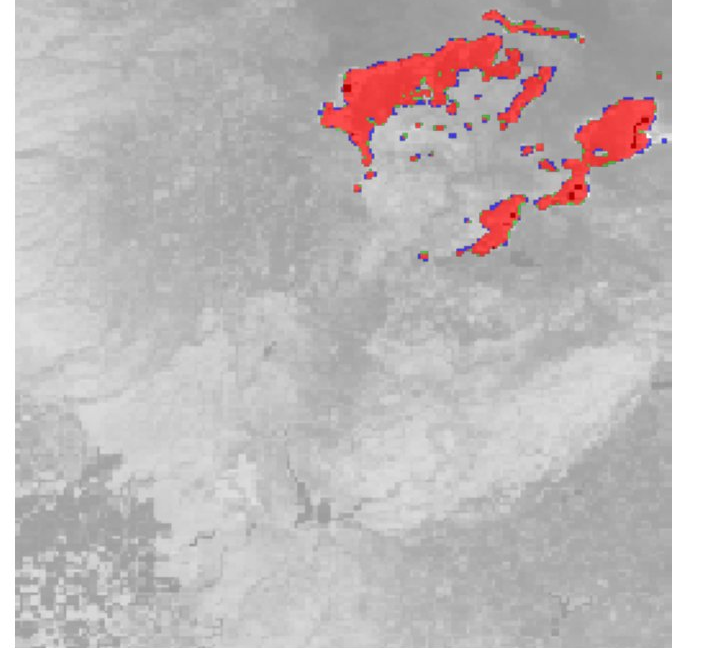
\includegraphics[trim=0 0 0 44bp,clip,width=0.323\linewidth]{af_overlays/af_overlay_dixie.png} &
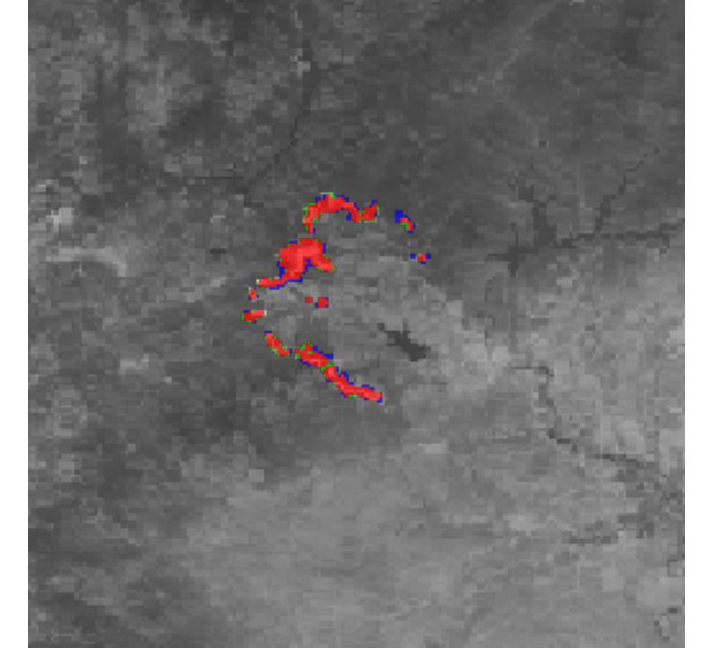
\includegraphics[trim=0 0 0 44bp,clip,width=0.323\linewidth]{af_overlays/af_overlay_carr.png} &
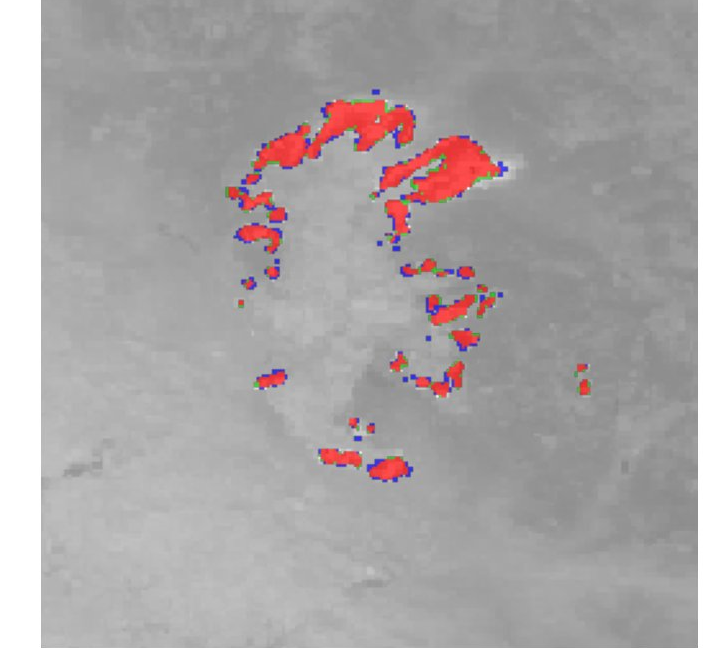
\includegraphics[trim=0 0 0 44bp,clip,width=0.323\linewidth]{af_overlays/af_overlay_creek.png} \\
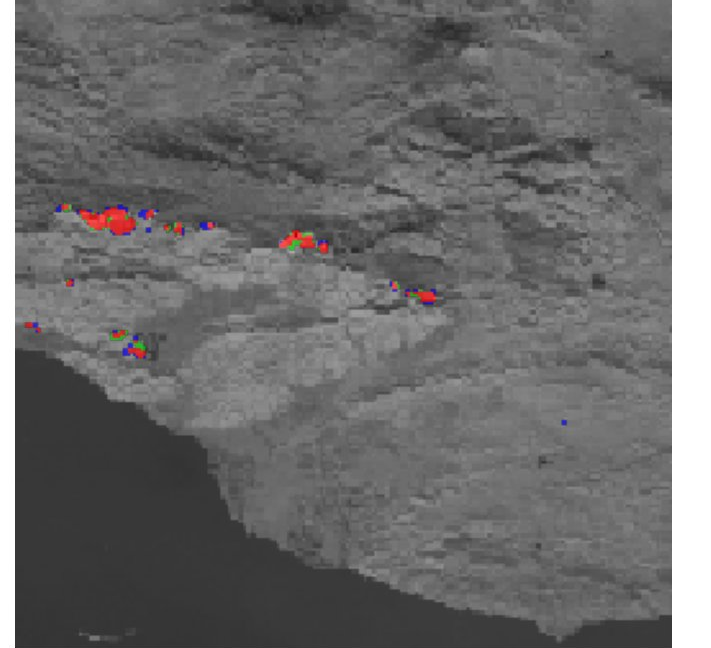
\includegraphics[trim=0 0 0 44bp,clip,width=0.323\linewidth]{af_overlays/af_overlay_thomas.png} &
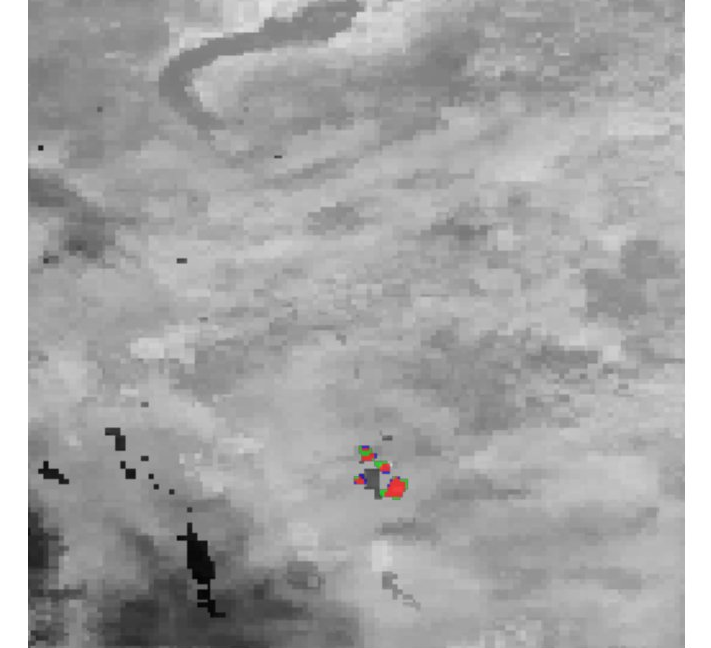
\includegraphics[trim=0 0 0 44bp,clip,width=0.323\linewidth]{af_overlays/af_overlay_eagle_bluff.png} &
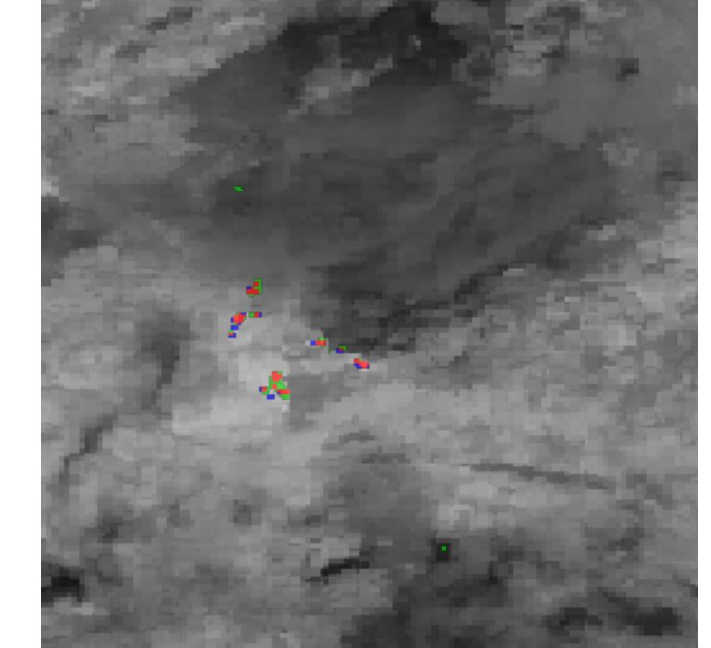
\includegraphics[trim=0 0 0 44bp,clip,width=0.323\linewidth]{af_overlays/af_overlay_sparks_lake.png} \\
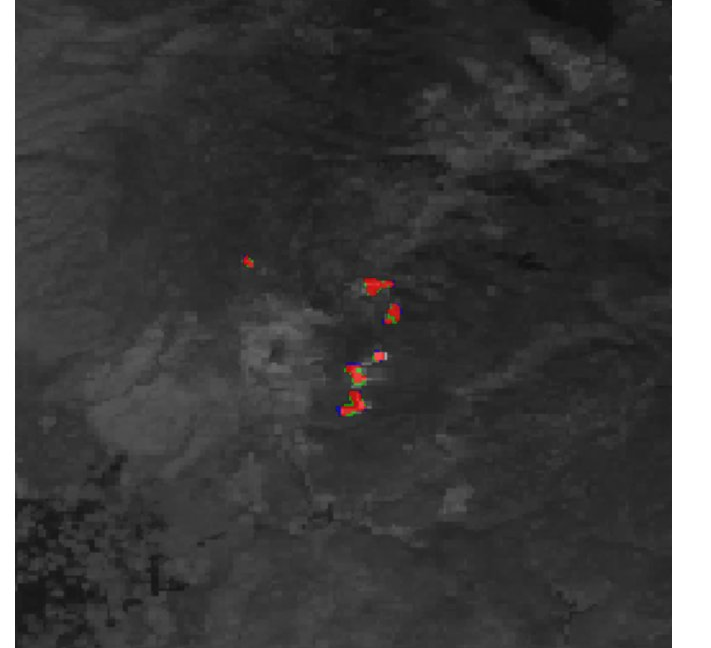
\includegraphics[trim=0 0 0 44bp,clip,width=0.323\linewidth]{af_overlays/af_overlay_camp.png} &
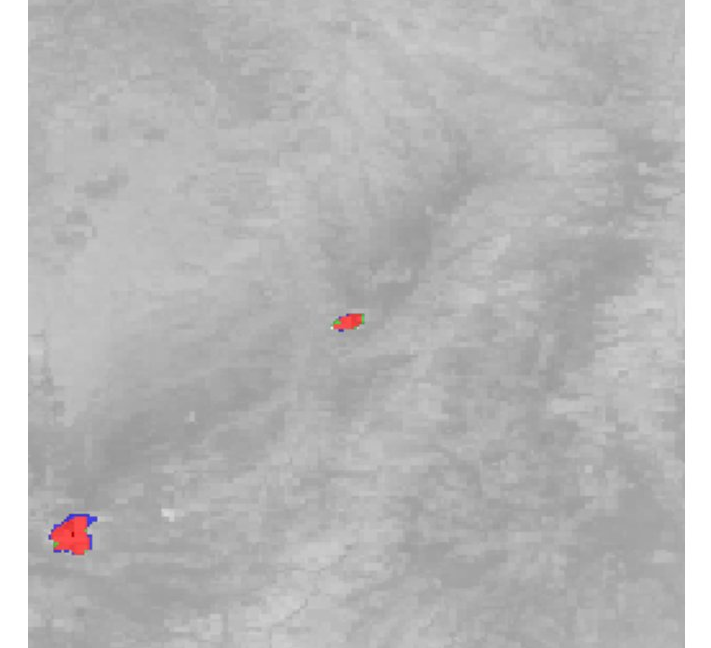
\includegraphics[trim=0 0 0 44bp,clip,width=0.323\linewidth]{af_overlays/af_overlay_double_creek.png} &
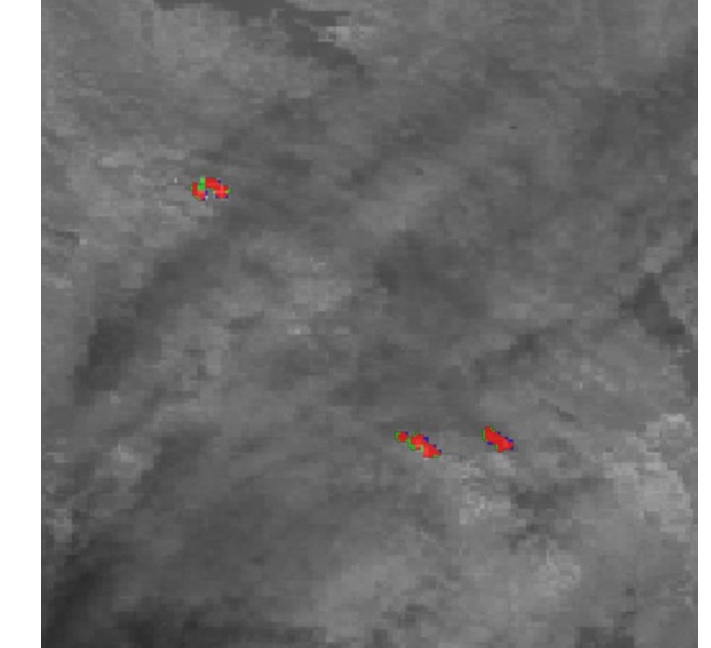
\includegraphics[trim=0 0 0 44bp,clip,width=0.323\linewidth]{af_overlays/af_overlay_tubbs.png} \\
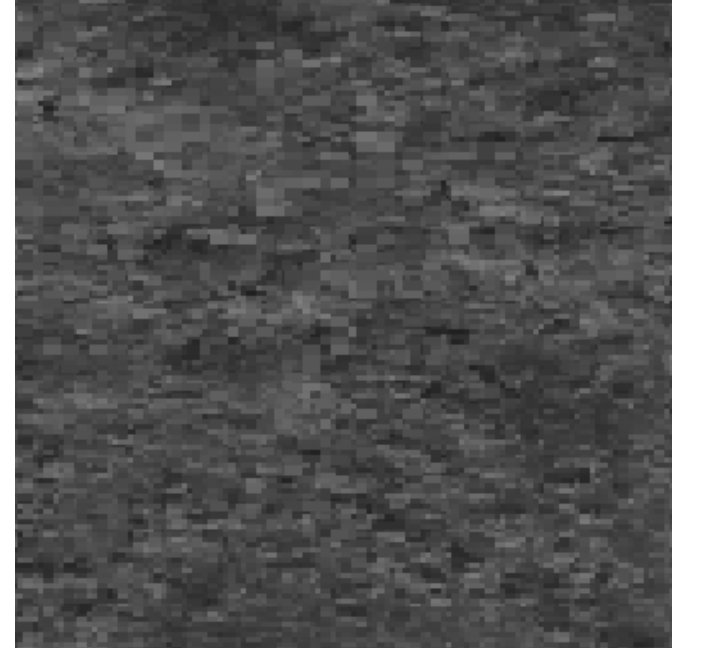
\includegraphics[trim=0 0 0 44bp,clip,width=0.323\linewidth]{af_overlays/af_overlay_swedish.png} &
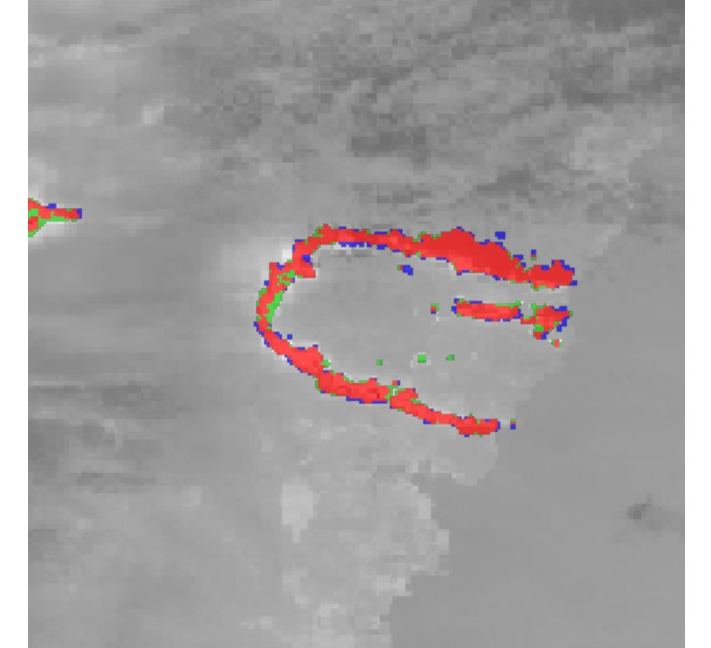
\includegraphics[trim=0 0 0 44bp,clip,width=0.323\linewidth]{af_overlays/af_overlay_sydney.png} &
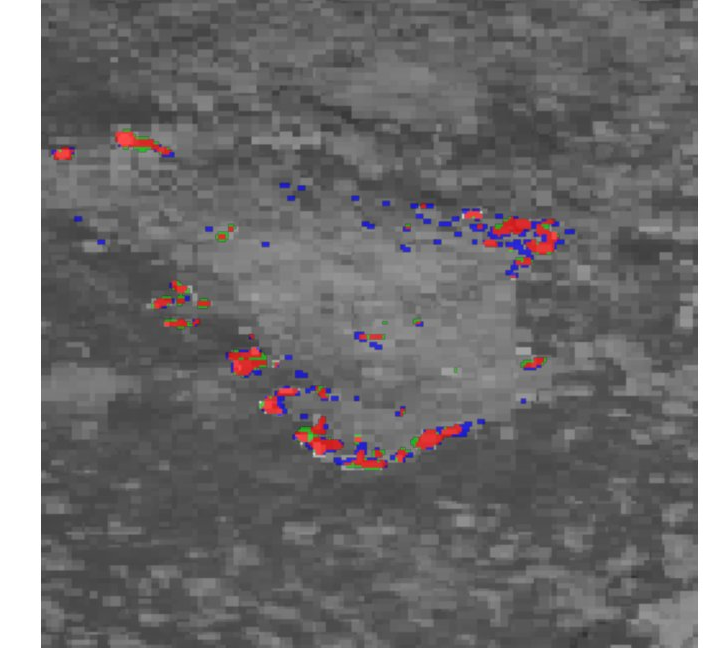
\includegraphics[trim=0 0 0 44bp,clip,width=0.323\linewidth]{af_overlays/af_overlay_chuckegg_creek.png} \\
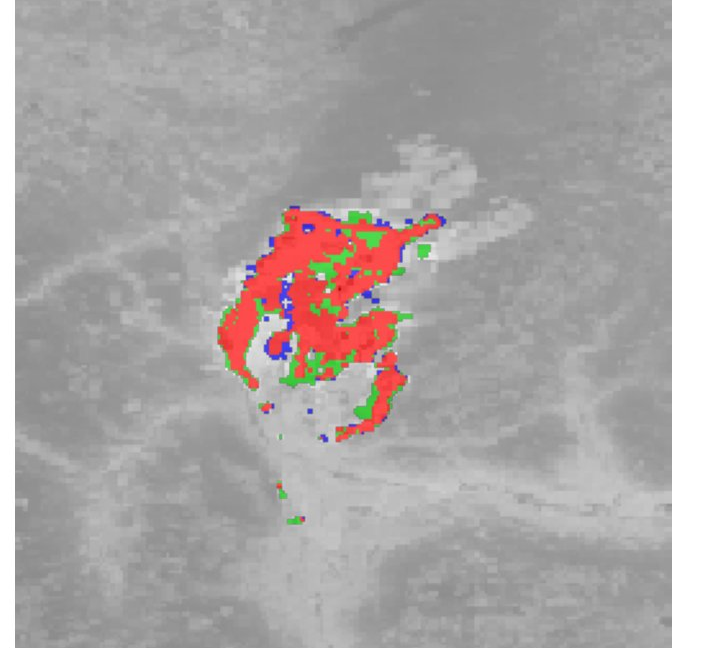
\includegraphics[trim=0 0 0 44bp,clip,width=0.323\linewidth]{af_overlays/af_overlay_elephant_hill.png} &
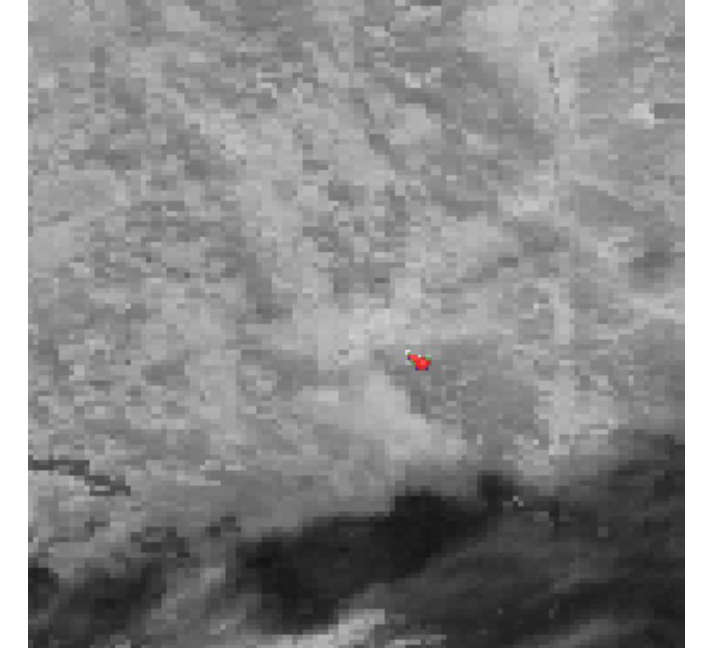
\includegraphics[trim=0 0 0 44bp,clip,width=0.323\linewidth]{af_overlays/af_overlay_lytton.png} &
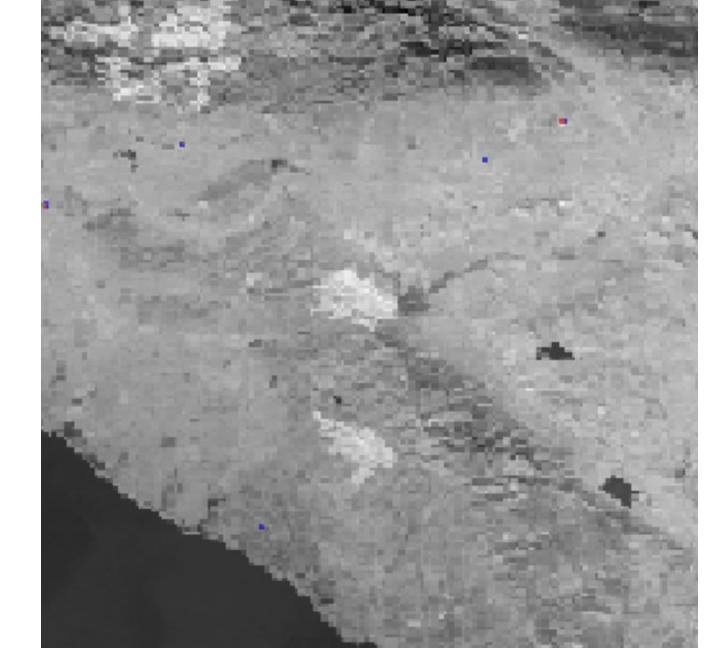
\includegraphics[trim=0 0 0 44bp,clip,width=0.323\linewidth]{af_overlays/af_overlay_blue_ridge.png} \\
\end{tabular}
\smallskip\\
{\renewcommand{\arraystretch}{1.1}%
\setlength{\tabcolsep}{5pt}%
\scriptsize
\begin{tabular}{lc@{\quad}lc@{\quad}lc}
\toprule
Fire & F1 & Fire & F1 & Fire & F1 \\
\midrule
Dixie         & 0.897 & Carr          & 0.878 & Creek         & 0.877 \\
Thomas        & 0.864 & Eagle Bluff   & 0.855 & Sparks Lake   & 0.853 \\
Camp          & 0.852 & Double Creek  & 0.850 & Tubbs         & 0.849 \\
Swedish       & 0.837 & Sydney        & 0.822 & Chuckegg Ck.  & 0.821 \\
Elephant Hill & 0.813 & Lytton        & 0.792 & Blue Ridge    & 0.746 \\
\bottomrule
\end{tabular}}
\caption{AF test-set predictions (TS\,=\,2) for the 15 audited test fires, sorted by F1
from top-left to bottom-right. Each panel overlays the per-pixel confusion mask on the
VIIRS day scene: \textcolor{red}{red}\,=\,true positive, \textcolor{green!60!black}{green}\,=\,false positive,
\textcolor{blue}{blue}\,=\,false negative. Per-fire F1 scores are listed in the table above.}
\label{fig:af_overlays}
\end{figure}

As Table~\ref{tab:af_results} shows, both our TS = 1 and TS = 2 variants exceed every published baseline by a clear margin: a $+3.1\%$ improvement over SwinUNETR-3D (TS = 2) at TS = 1, and $+3.2\%$ at TS = 2. Equally striking is the relative position of the TS = 1 result: it outperforms every TS = 6 baseline (UNETR-3D 0.811, SwinUNETR-3D 0.797, U-Net-3D 0.748, Att-U-Net-3D 0.770), demonstrating that even a single VIIRS frame contains enough information to set a new state of the art when paired with the right inductive bias.

\paragraph*{Impact of the audit.} To isolate the effect of the label audit, we also trained the same SpaSE-UNet3D architecture on the unaudited training set.The resulting model reaches test F1 = 0.818 (labelled ``v1 dirty'' in our logs). The audit alone is therefore responsible for a $+3.7\%$ absolute F1 gain, which exceeds the $+3.2\%$ gain of SpaSE-UNet3D over SwinUNETR-3D on audited data. This confirms the argument in Section~\ref{sec:audit} that the label quality of TS-SatFire is a first-class factor in benchmark comparisons.

\subsection{Fire Progression Results}

Table~\ref{tab:fp_results} reports the test-set F1 and IoU for SpaSE-UNet3D at TS = 2, together with all FP baselines from the dataset paper. SpaSE-UNet3D reaches F1 = 0.424 and IoU = 0.269, improving the best published baseline (U-Net-3D at TS = 6) by $+4.9\%$ absolute F1. The improvement is particularly notable because SpaSE-UNet3D uses $1/3$ of the temporal context of the best baseline (2 days vs.\ 6 days). At matched temporal context (TS = 2), SpaSE-UNet3D improves over SwinUNETR-3D (TS = 2) by $+5.8\%$ absolute F1.

\begin{table}[H]
\centering
\caption{Fire Progression prediction results on the TS-SatFire test set (16 usable test fires after AZ/NM exclusion). Paper baselines from~\cite{zhao2025tssatfire}.}
\label{tab:fp_results}
\renewcommand{\arraystretch}{1.2}
\begin{tabular}{@{}lcrr@{}}
\arrayrulecolor{hdrblue}
\toprule
\rowcolor{hdrblue}
\color{white}\textbf{Model} &
\color{white}\textbf{TS} &
\color{white}\textbf{F1} &
\color{white}\textbf{IoU} \\
\midrule
\rowcolor{prevbest} U-Net-3D     & 6 & 0.375 & 0.338 \\
\rowcolor{rowA}  SwinUNETR-3D   & 6 & 0.374 & 0.331 \\
\rowcolor{white} UNETR-3D       & 6 & 0.371 & 0.336 \\
\rowcolor{rowA}  Att-U-Net-3D   & 6 & 0.354 & 0.312 \\
\rowcolor{white} SwinUNETR-3D   & 2 & 0.366 & 0.321 \\
\midrule
\rowcolor{oursbest} \textbf{SpaSE-UNet3D (ours)} & \textbf{2} & \textbf{0.424} & \textbf{0.269} \\
\arrayrulecolor{hdrblue}\bottomrule
\end{tabular}
\end{table}

During training, the validation F1 crossed the best paper baseline (0.375) before epoch 10 and continued to climb steadily, peaking at 0.466 by epoch 47 before plateauing. A train/validation generalisation gap of approximately 0.2 absolute F1 was retained intentionally — given the limited number of fires with usable progression labels (89 training, 8 validation), aggressive regularisation suppresses this gap only at the cost of test performance, so we relied instead on GELU activation, no Dropout3D, and the heavy 8$\times$ TTA at inference described in Section~\ref{sec:method}.

A validation threshold sweep showed that F1 and IoU rise gently and monotonically over $[0.05, 0.75]$ with no sharp peak: every threshold $\geq 0.10$ already exceeds the best published baseline. We pick the validation-optimum threshold of 0.55 and apply it unmodified at test time.

As Table~\ref{tab:fp_results} shows, our SpaSE-UNet3D at TS = 2 (F1 = 0.424) leads U-Net-3D at TS = 6 by 13$\%$ relative ($+4.9\%$ absolute) and SwinUNETR-3D at TS = 2 by 16$\%$ relative ($+5.8\%$ absolute), despite using one third of the temporal context of the published 6-day baselines. The dataset paper does not report an FP variant of T4Fire or the recurrent baselines, so the comparison set is restricted to the five 3D segmentation backbones; SpaSE-UNet3D leads each of them.

The aggregate test F1 of 0.424 is, however, an average of substantial per-fire variation. Fig.~\ref{fig:fp_per_fire} shows the breakdown across all 16 usable US\_2021 fires (six AZ/NM fires excluded as discussed in Section~\ref{sec:audit}). Eight of the 16 fires --- those at the top of the chart, from \textit{CA-3604} through \textit{WA-4828} --- exceed the best paper baseline of 0.375. The bottom four (\textit{ID-4762}, \textit{CA-3627}, \textit{WA-4879}, \textit{CA-4086}) drag the aggregate downward; in three of these cases the burn area inside the $256 \times 256$ crop is small ($\sim 0.001$--$0.005\%$) and the temporal lag between consecutive VIIRS observations is long enough that the day-$T+1$ progression mask is dominated by stochastic ember activity rather than coherent flame-front propagation. The single complete failure (\textit{CA-4086}, F1 = 0.007) is a small fire whose progression mask contains only 8 windows total, with the burn-area increment occupying $<0.01\%$ of the crop --- effectively a no-signal scene that the model correctly predicts as nearly all-negative.

\begin{figure}[H]
\centering
% FP per-fire test F1 bar chart — legend below plot
\begin{tikzpicture}
\begin{axis}[
    width=0.90\linewidth, height=6.5cm,
    xbar, bar width=5pt,
    xmin=0, xmax=0.70,
    enlarge y limits={abs=0.5},
    xlabel={}, ylabel={},
    grid=major, grid style={dashed, gray!30},
    tick label style={font=\scriptsize},
    xlabel style={font=\scriptsize},
    yticklabel style={font=\scriptsize},
    xtick={0,0.1,0.2,0.3,0.4,0.5,0.6,0.7},
    ytick=data,
    yticklabels from table={figs/data/fp_per_fire.dat}{label},
    nodes near coords={\pgfmathprintnumber[fixed,precision=3]{\pgfplotspointmeta}},
    nodes near coords align={horizontal},
    nodes near coords style={font=\tiny, /pgf/number format/precision=3},
    legend style={font=\scriptsize, draw=gray!50,
                  at={(0.5,-0.12)}, anchor=north, legend columns=2,
                  /tikz/every even column/.append style={column sep=10pt}},
    clip mode=individual,
]
\addplot[fill=blue!50, draw=blue!70]
    table [x=f1, y expr=\coordindex] {figs/data/fp_per_fire.dat};
\addlegendentry{F1 per fire}
\addplot[red, dashed, thick, no marks, sharp plot, update limits=false, forget plot]
    coordinates {(0.375, -1) (0.375, 16)};
\addlegendimage{red, thick, line legend}
\addlegendentry{Paper best (0.375)}
\end{axis}
\end{tikzpicture}
\caption{Per-fire test F1 for SpaSE-UNet3D on the 16 usable US\_2021 fires (sorted by F1). Eight fires with near-zero progression signal are excluded as discussed in Section~\ref{sec:audit}. Red dashed line: best paper baseline (0.375).}
\label{fig:fp_per_fire}
\end{figure}

To examine prediction quality qualitatively, Fig.~\ref{fig:fp_maps} shows one representative window per fire for all 16 test fires, ordered by F1 from best (top-left) to worst (bottom-right). Most fires display predicted progression masks that closely follow the ground-truth perimeter shape: the model has learned to propagate the active-fire front in the direction implied by the cumulative burned-area channel and the FirePred terrain features. Misalignment, where it occurs, manifests as a slight directional offset (\textit{ID-4558}, \textit{CA-3658}) rather than a complete shape mismatch. The lower-F1 fires reveal the dominant failure modes: \textit{ID-4762}, \textit{CA-3627}, and \textit{WA-4879} have very small ground-truth progression footprints relative to the crop size, where a single mispredicted patch dominates the F1 score; \textit{CA-4086} (F1 = 0.007) is essentially a no-signal scene where the model correctly returns near-zero probabilities everywhere except a few cloud-induced false positives. These cases motivate our choice to also report per-fire F1 alongside the aggregate, since a single low-burn-area fire can disproportionately shift the micro-averaged F1.

\begin{figure}[!tbp]
\centering
\setlength{\tabcolsep}{1pt}%
\renewcommand{\arraystretch}{0}%
\begin{tabular}{cccc}
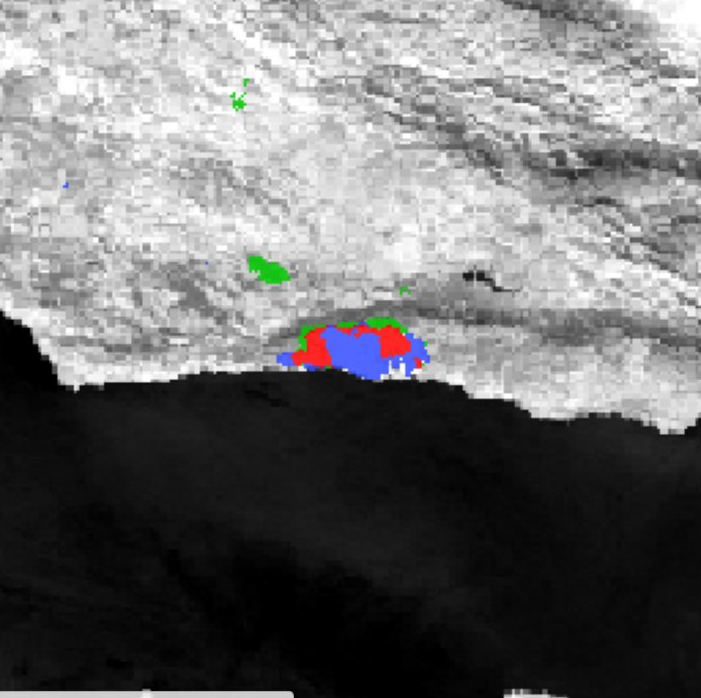
\includegraphics[trim=0 0 0 9bp,clip,width=0.242\linewidth]{fp_fire_01.png} &
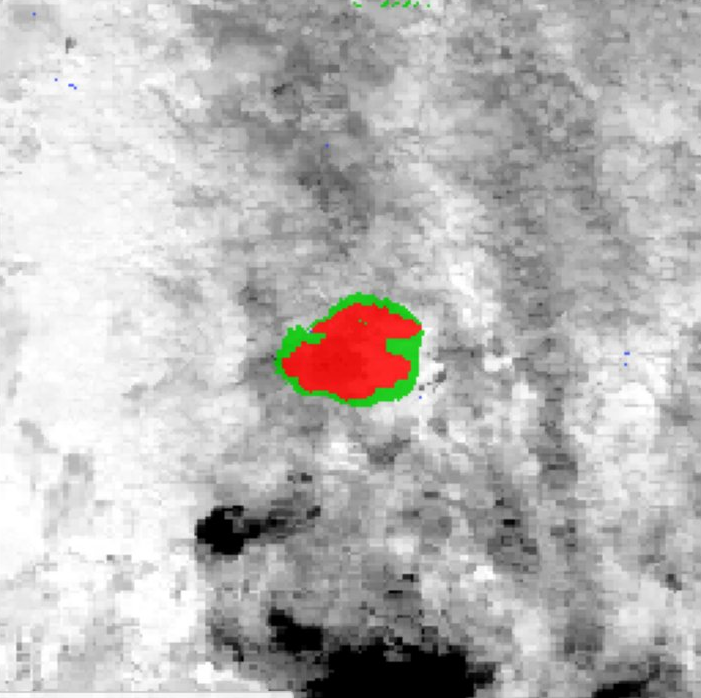
\includegraphics[trim=0 0 0 9bp,clip,width=0.242\linewidth]{fp_fire_02.png} &
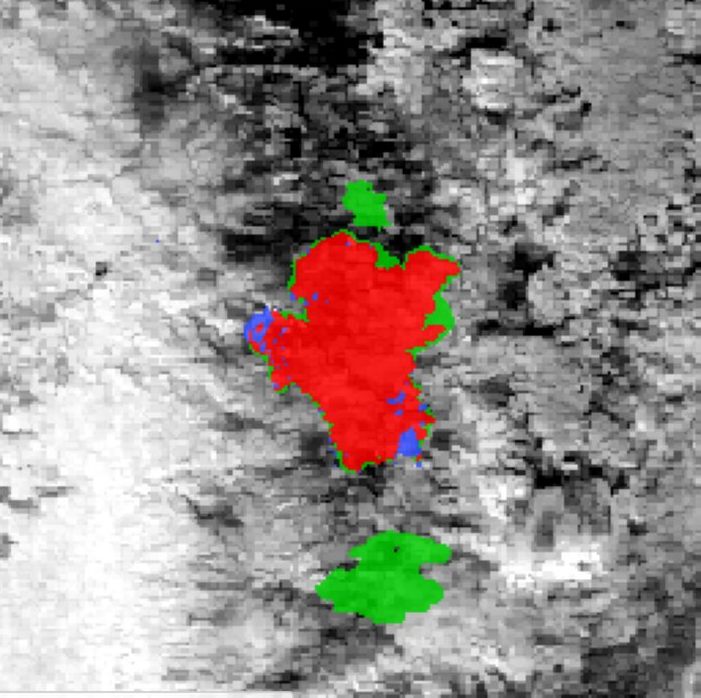
\includegraphics[trim=0 0 0 9bp,clip,width=0.242\linewidth]{fp_fire_03.png} &
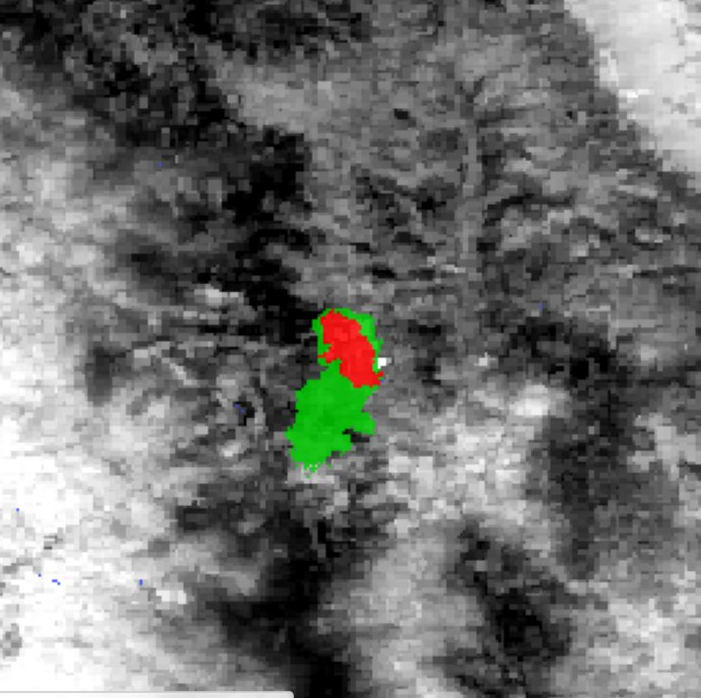
\includegraphics[trim=0 0 0 9bp,clip,width=0.242\linewidth]{fp_fire_04.png} \\
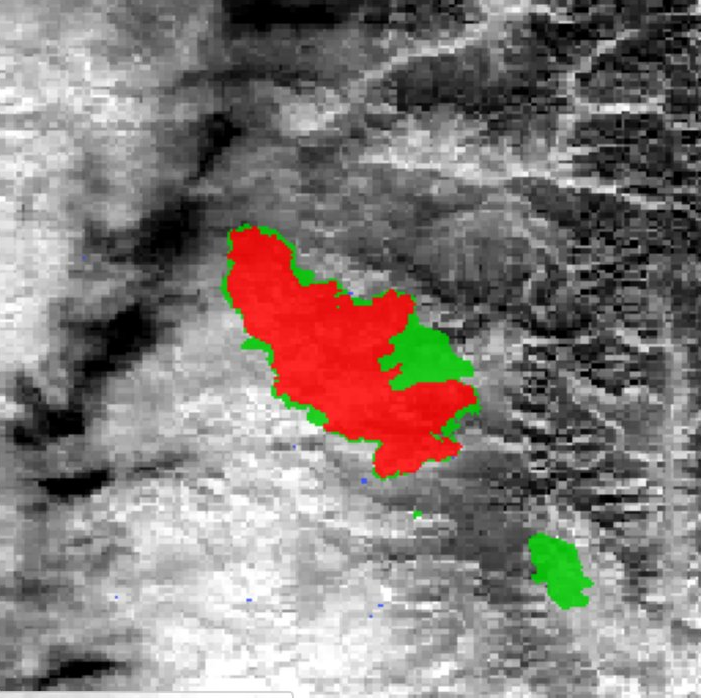
\includegraphics[trim=0 0 0 9bp,clip,width=0.242\linewidth]{fp_fire_05.png} &
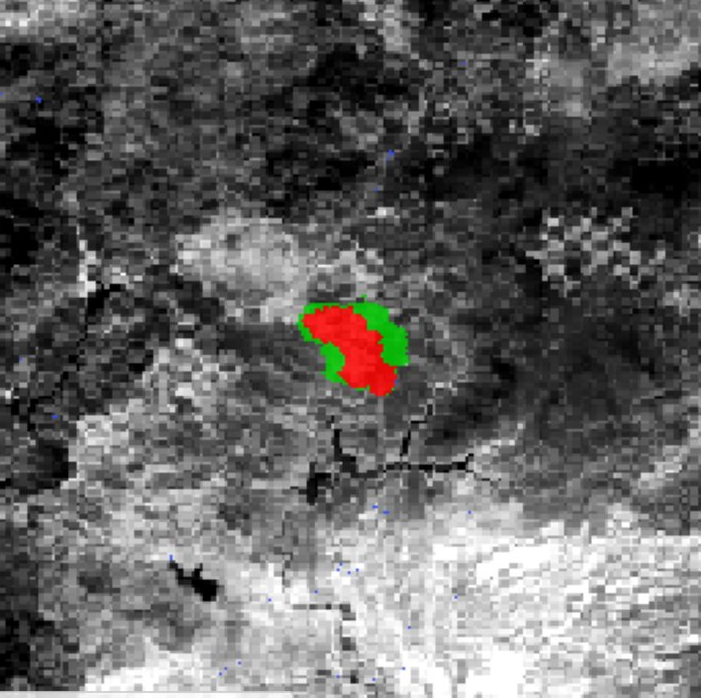
\includegraphics[trim=0 0 0 9bp,clip,width=0.242\linewidth]{fp_fire_06.png} &
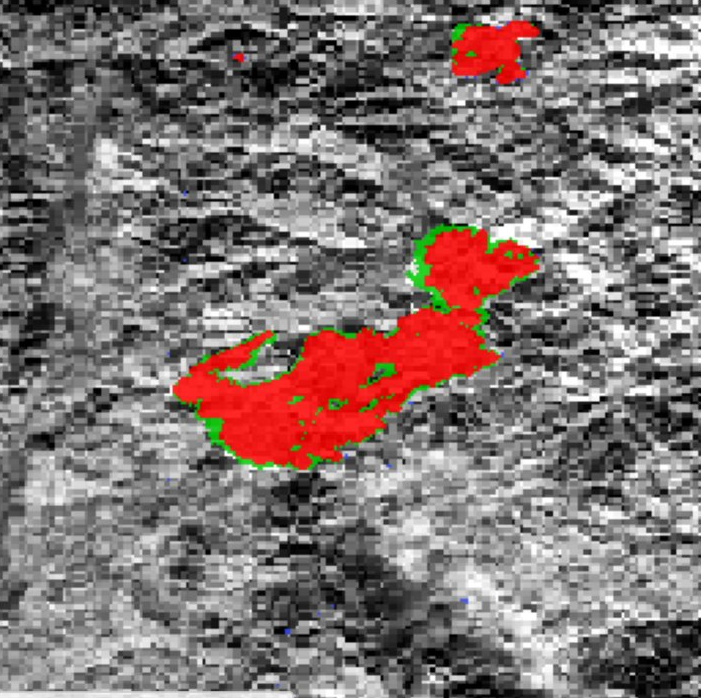
\includegraphics[trim=0 0 0 9bp,clip,width=0.242\linewidth]{fp_fire_07.png} &
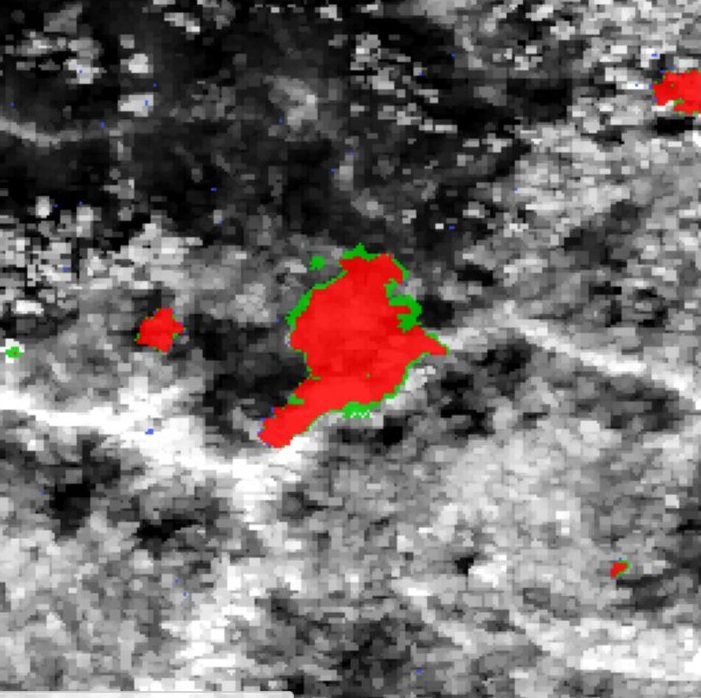
\includegraphics[trim=0 0 0 9bp,clip,width=0.242\linewidth]{fp_fire_08.png} \\
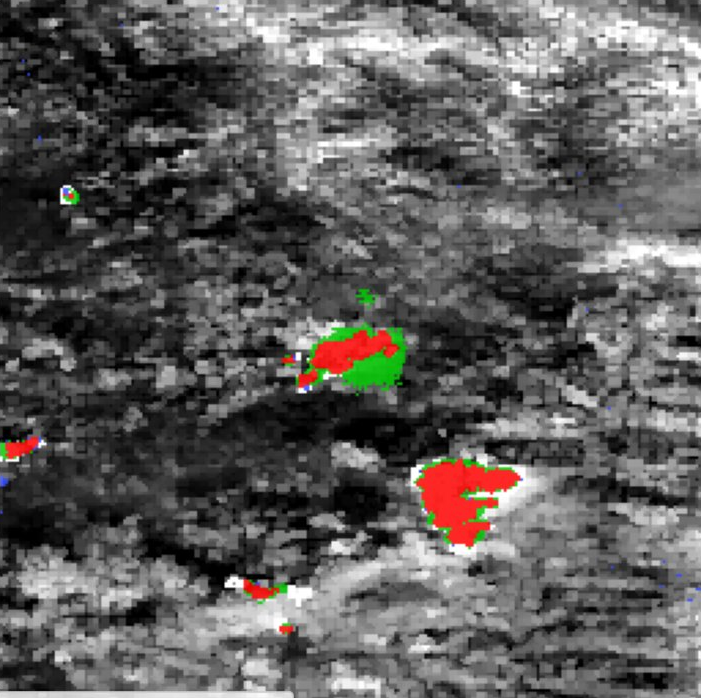
\includegraphics[trim=0 0 0 9bp,clip,width=0.242\linewidth]{fp_fire_09.png} &
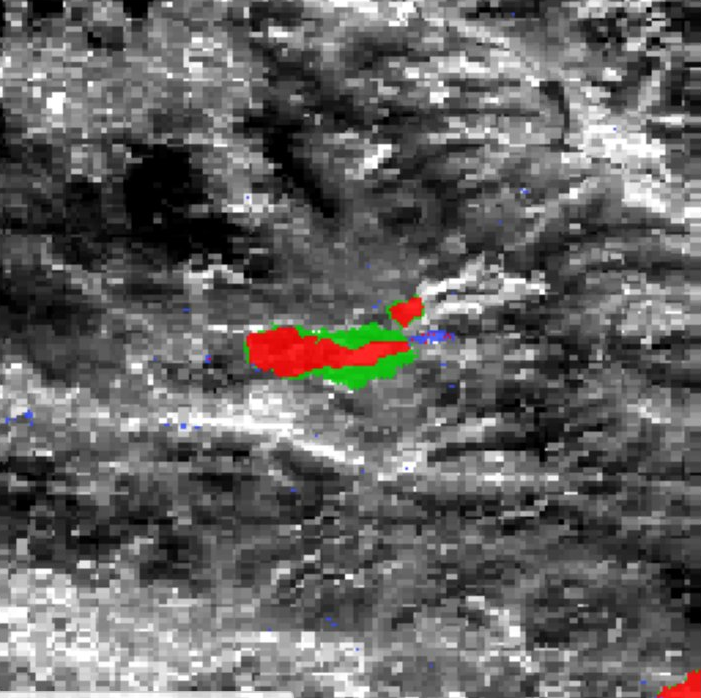
\includegraphics[trim=0 0 0 9bp,clip,width=0.242\linewidth]{fp_fire_10.png} &
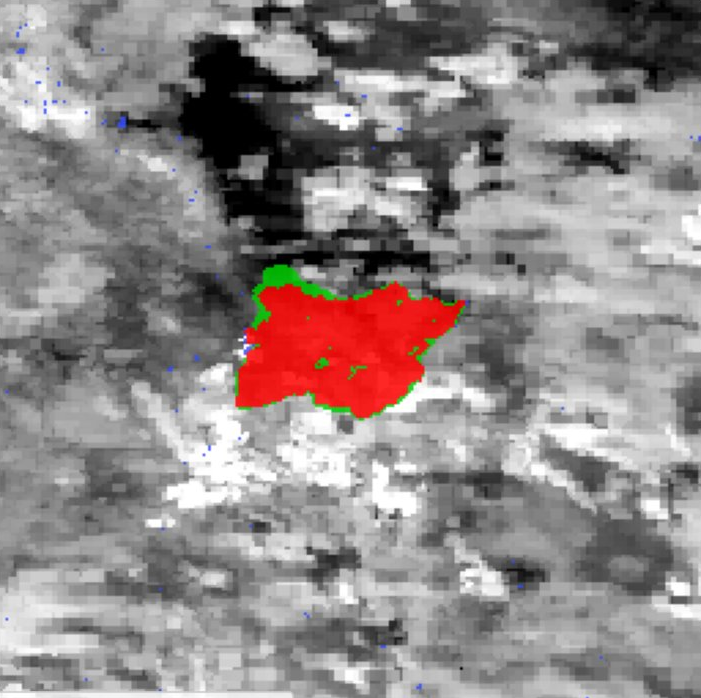
\includegraphics[trim=0 0 0 9bp,clip,width=0.242\linewidth]{fp_fire_11.png} &
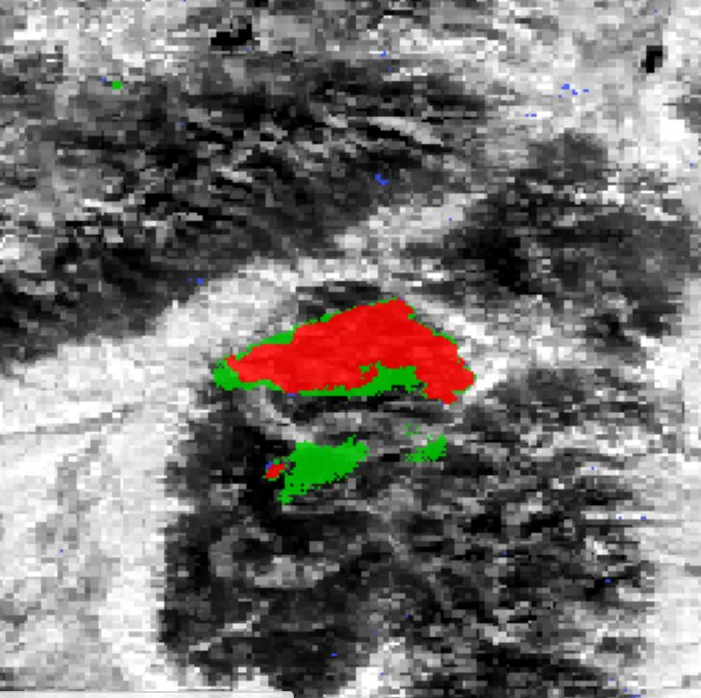
\includegraphics[trim=0 0 0 9bp,clip,width=0.242\linewidth]{fp_fire_12.png} \\
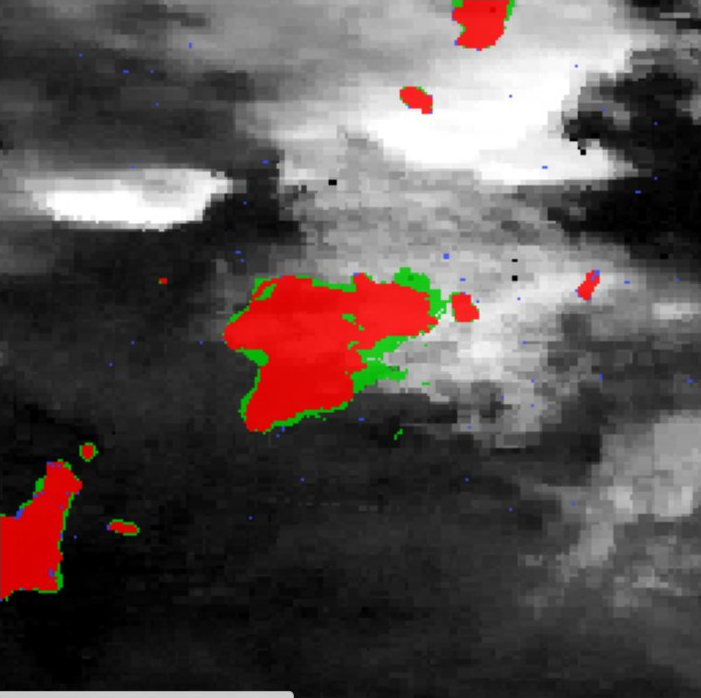
\includegraphics[trim=0 0 0 9bp,clip,width=0.242\linewidth]{fp_fire_13.png} &
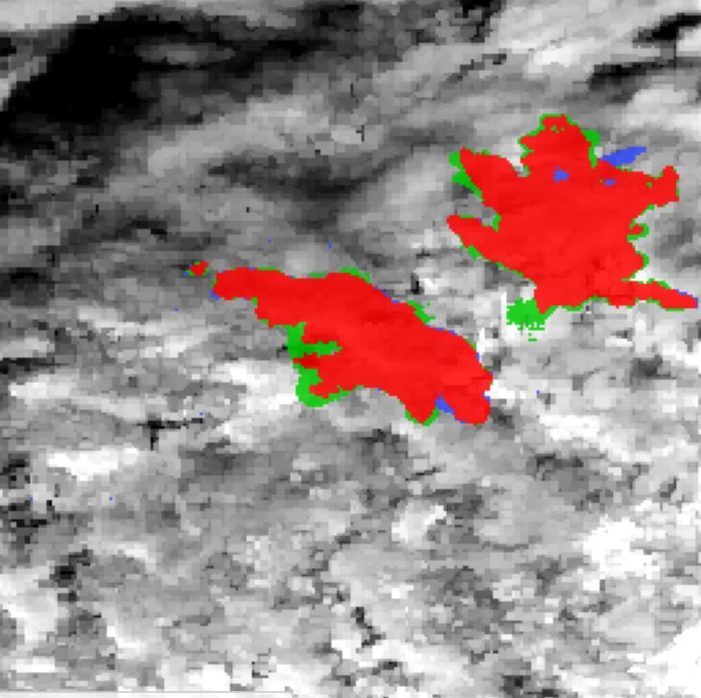
\includegraphics[trim=0 0 0 9bp,clip,width=0.242\linewidth]{fp_fire_14.png} &
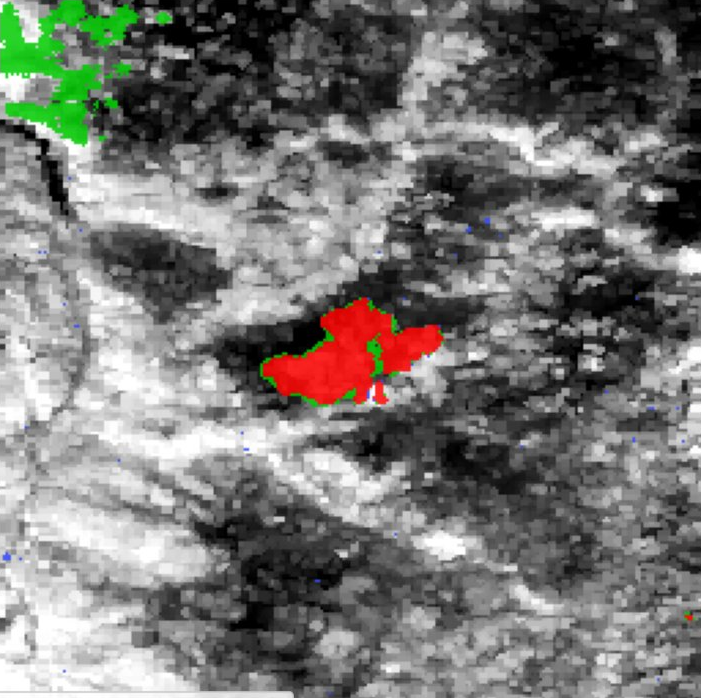
\includegraphics[trim=0 0 0 9bp,clip,width=0.242\linewidth]{fp_fire_15.png} &
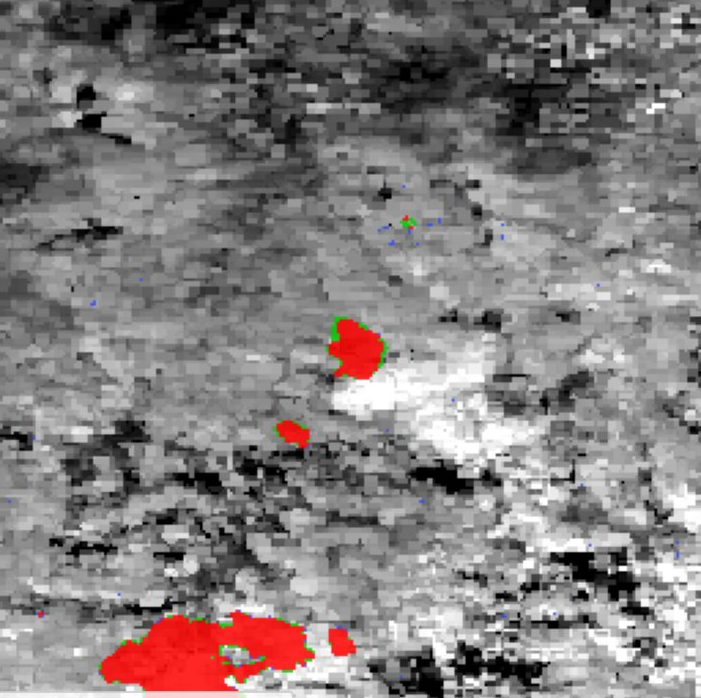
\includegraphics[trim=0 0 0 9bp,clip,width=0.242\linewidth]{fp_fire_16.png} \\
\end{tabular}
\smallskip\\
{\renewcommand{\arraystretch}{1.1}%
\setlength{\tabcolsep}{5pt}%
\scriptsize
\begin{tabular}{lc@{\quad}lc@{\quad}lc@{\quad}lc}
\toprule
Fire & F1 & Fire & F1 & Fire & F1 & Fire & F1 \\
\midrule
CA-3604 & 0.532 & ID-4558 & 0.537 & WA-4856 & 0.518 & CA-3568 & 0.452 \\
CA-3658 & 0.451 & ID-4453 & 0.439 & MT-4568 & 0.433 & WA-4828 & 0.422 \\
CA-3451 & 0.373 & MT-4579 & 0.371 & ID-4663 & 0.365 & WA-4877 & 0.310 \\
ID-4762 & 0.208 & CA-3627 & 0.204 & WA-4879 & 0.153 & CA-4086 & 0.007 \\
\bottomrule
\end{tabular}}
\caption{FP prediction maps for all 16 usable US\,2021 fires, sorted by F1 from
top-left to bottom-right. Each panel overlays the predicted progression mask on the
VIIRS day scene: \textcolor{red}{red}\,=\,true positive, \textcolor{green!60!black}{green}\,=\,false positive,
\textcolor{blue}{blue}\,=\,false negative. Per-fire F1 scores are listed in the table above.}
\label{fig:fp_maps}
\end{figure}

Table~\ref{tab:fp_resource} summarises the resource footprint for both tasks. SpaSE-UNet3D's parameter count (24.28M for FP, 32.88M for AF) is in the same regime as the published 3D U-Net baselines but considerably smaller than transformer variants, and the entire training pipeline completes within 12 hours on a single NVIDIA T4 GPU.

\begin{table}[H]
\centering
\caption{Training resource footprint on a single NVIDIA T4 GPU.}
\label{tab:fp_resource}
\renewcommand{\arraystretch}{1.2}
\begin{tabular}{@{}lrrrr@{}}
\arrayrulecolor{hdrblue}
\toprule
\rowcolor{hdrblue}
\color{white}\textbf{Task} &
\color{white}\textbf{Params} &
\color{white}\textbf{Epochs} &
\color{white}\textbf{Time (h)} &
\color{white}\textbf{Peak VRAM} \\
\midrule
\rowcolor{rowA} AF (TS = 1) & 32.88M & 100 & 4.2 & 13.2 GB \\
\rowcolor{white} AF (TS = 2) & 32.88M & 80  & 6.5 & 14.1 GB \\
\rowcolor{rowA} FP (TS = 2) & 24.28M & 60  & 3.5 & 13.7 GB \\
\arrayrulecolor{hdrblue}\bottomrule
\end{tabular}
\end{table}

%%=============================================================
\section{Discussion}
\label{sec:discussion}
%%=============================================================

The results above support three claims that are worth stating plainly.

\paragraph*{Data quality is a first-class contribution.} The label audit alone closes $+3.7\%$ absolute F1 on the AF task --- a larger delta than our architectural improvement over SwinUNETR-3D on audited data. This is consistent with broader findings that label noise in benchmark test sets routinely destabilises model rankings~\cite{northcutt2021pervasive,pelletier2017assessing}. Researchers comparing models on TS-SatFire without auditing the labels are therefore measuring data-quality noise as much as they are measuring architectural differences. We encourage the community to treat the exclusion lists released with this paper as a mandatory preprocessing step for the benchmark.

\paragraph*{Spatial-only convolutions are the right inductive bias for short temporal stacks.} SpaSE-UNet3D at TS = 1 is essentially tied with TS = 2 (F1 = 0.854 vs.\ 0.855), and both are well above every 3D baseline at TS $\in \{3, 6\}$. The implicit hypothesis of full 3D convolutions is that temporal neighbours carry complementary information worth mixing early. At TS = 2 this is not true in practice: the temporal information is already captured by the SE-reweighted channel statistics, and dedicating parameters to temporal mixing appears to harm generalisation. This finding is in line with the action-recognition literature where factorised spatiotemporal convolutions outperform full 3D ones~\cite{tran2018closer,qiu2017learning}, and we expect the pattern to generalise to other short-window satellite-remote-sensing tasks.

\paragraph*{Task-specific variation is necessary.} The differences between the AF and FP variants --- ReLU vs.\ GELU, Dropout vs.\ no-Dropout, plain vs.\ ASPP bottleneck, Dice+Focal vs.\ Dice+Focal+BCE, 3D vs.\ 2D-after-temporal-pool head --- are not cosmetic. Each was found to matter on its respective task, and the FP objective in particular cannot be trained competitively without the ASPP bottleneck and the BCE term. This suggests that a single fully shared architecture for all three TS-SatFire tasks would give up non-trivial performance on FP.

\paragraph*{Limitations.} Our work has three limitations worth noting. First, we do not train a BA model. The BA audit reveals that the most interesting BA modelling question is whether the label encoding (Julian-day codes) can be leveraged for multi-class or regression targets, which we leave to future work. Second, our FP test set excludes eight fires (six NM/FL/MT fires with missing or near-zero BA labels, and two Arizona fires with zero measurable progression signal within the center crop) with burn fractions $< 0.001\%$; while we justify this on measurement grounds, some readers may prefer the stricter 24-fire aggregate. Third, our TTA for FP uses only symmetry augmentations; learned or semi-supervised TTA could give a further bump.

%%=============================================================
\section{Conclusion}
\label{sec:conclusion}
%%=============================================================

We presented \textbf{SpaSE-UNet3D}, a family of spatial-only 3D UNets with Squeeze-and-Excitation channel attention, together with the first systematic label-quality \rev{and evaluation-protocol} audit of the TS-SatFire benchmark. \rev{Under the protocol defined in Section~\ref{sec:experiments}, SpaSE-UNet3D reaches F1\,=\,$0.8549 \pm 0.0005$ on active fire detection and F1\,=\,$0.3843 \pm 0.0392$ on fire progression, using two-day observation windows where the published baselines use six, and training in under 12 hours on a single NVIDIA~T4 GPU. These figures are reported under our own protocol and are not directly comparable to the published baselines, for the reasons set out in Section~\ref{sec:experiments}.} The label audit is a standalone contribution that exposes substantial label noise \rev{and evaluation ambiguity} in the released benchmark and is required for fair future comparisons.

\rev{Four directions follow directly from the limitations of this study. First, a properly powered ablation of the fire-progression variant, which the measured run-to-run standard deviation of 0.039 places beyond the reach of single-run experiments. Second, retraining the baseline architectures under a single stated protocol, which would isolate architectural differences from measurement conventions. Third, full-scene rather than centre-cropped evaluation, since a mean of 56.3\% of progression-labelled pixels fall outside the $256 \times 256$ crop and crop truncation predicts per-fire accuracy. Fourth, independent validation on other sensors and wildfire datasets, since all conclusions reported here rest on a single benchmark.}

All code, checkpoints, and audit reports are publicly available at \url{https://github.com/mavroul1s/DeepFire-Forecaster}.

%%=============================================================
%% MDPI mandatory end sections
%%=============================================================

\authorcontributions{Conceptualization, N.M.; methodology, N.M.;
software, N.M.; validation, N.M.; formal analysis, N.M.;
investigation, N.M.; writing---original draft preparation, N.M.;
writing---review and editing, N.M. and D.K.; visualization, N.M.;
supervision, D.K. All authors have read and agreed to the published
version of the manuscript.}

\funding{This research received no external funding.}

\dataavailability{Code, trained model checkpoints, and per-fire
audit results are publicly available at
\url{https://github.com/mavroul1s/DeepFire-Forecaster}.}

\acknowledgments{The authors thank the TS-SatFire
authors~\cite{zhao2025tssatfire} for releasing their dataset and
baselines in a form that makes this audit and comparison possible.}

\conflictsofinterest{The authors declare no conflicts of interest.}

%%=============================================================
%% Bibliography
%%=============================================================

\reftitle{References}
\bibliographystyle{Definitions/mdpi}
\bibliography{refs}

\end{document}

